\documentclass[12pt,a4paper,oneside]{book}
\usepackage[english]{babel}
\usepackage{amsmath}
\usepackage{amsthm}
\usepackage{amsfonts}
\usepackage{amssymb}
\usepackage{graphicx}
\usepackage{geometry}
\usepackage{array}
\usepackage{longtable}
\usepackage[percent]{overpic}
\usepackage{tikz}
\usepackage[titletoc]{appendix}
\usepackage[round]{natbib}
\usepackage{titlesec}
\usepackage{amsmath}
\usepackage{bm}
\usepackage{mathtools}
\usepackage{geometry}
\usepackage{float}
\usepackage[hyphens]{url}
\usepackage{apacite}
\usepackage[capposition=top]{floatrow}
\usepackage{caption}
\usepackage[labelfont=bf]{caption}
\usepackage[flushleft]{threeparttable}
\geometry{bindingoffset=0cm,margin=1in,hratio=1:1}
%\usepackage[usenames,dvipsnames,svgnames,table]{xcolor}
\definecolor{kuleuven}{RGB}{29,141,176}
\definecolor{kuleuven1}{RGB}{82,189,236}
\usepackage{titlesec}
\usepackage{listings}
\titlespacing*{\section}
{0pt}{1ex}{1.5ex}
\titlespacing*{\subsection}
{0pt}{0ex}{0.5ex}
\titlespacing*{\subsubsection}
{0pt}{0.5ex}{0ex}
\setlength\parindent{0pt}
\newcommand{\nocontentsline}[3]{}
\newcommand{\tocless}[2]{\bgroup\let\addcontentsline=\nocontentsline#1{#2}\egroup}

\newcommand\numberthis{\addtocounter{equation}{1}\tag{\theequation}}

\newcommand{\R}{\mathbb{R}}

\allowdisplaybreaks

\makeindex

\begin{document}
%Start
\frontmatter
\newgeometry{textwidth=540pt,textheight=780pt,top=20pt,left=20pt,right=20pt}
\begin{titlepage}

\begin{figure}[t]{%
      \begin{overpic}[width=1\textwidth]{Picture1.png}
         \put(46,4){\color{white}\normal{\textbf{FACULTY OF ECONOMICS AND BUSINESS}}}
      \end{overpic}
    }
\end{figure}

\vspace*{4.5cm}
\hspace{0.75cm}{\color{kuleuven1}{\Huge Eurobonds \& Sovereign Risk }}

\vspace*{0.45cm}
\hspace{0.75cm}{\large     An Analysis of Eurobonds \& Bargain Power in a Sovereign Default Model}

\begin{figure}[b]
  %\centering
   \begin{minipage}[c]{0.4\textwidth}  {%
      \begin{overpic}[width=0.9\textwidth]{Picture2.png}
         \put(70,45){\begin{minipage}[c]{1.80\textwidth}
\begin{flushright}

{\Large Stijn Vermeulen} \linebreak
{Student number: 0748636} \linebreak

\textbf{{\large Thesis submitted to obtain \linebreak
the degree of}} \linebreak

%!!!IMPORTANT!!!:
%indicate the appropriate title of your master and major. Check the website https://feb.kuleuven.be/studentenportaal/contact/masterproef-leuven
{\large Master of Advanced Studies in Economics}\linebreak
\linebreak
\textbf{{\large Promoter:}}   Prof. Michal Kobielarz\linebreak


%\linebreak

\textbf{{\large Academic year:}} {\large 2019-2020}
\linebreak
\end{flushright}
  \end{minipage}}
      \end{overpic}
    }
  \end{minipage}


\begin{picture}(540,0.2)
\put(0,0){\colorbox{kuleuven1}{\makebox(540,0.2){}}}
\end{picture}
\end{figure}

\end{titlepage}
%%%%%%%%%%%%%%%%%%%%%%%%%%%%%%%%%%%%%%%%%%%%%%%%%%%%%%%%%%%%%%%%%%%%%%%%%%%%%%%%%%%%%%%%%%%%%%%%%%%% 
%Abstract
\frontmatter\pagenumbering{Roman}
\restoregeometry
\setcounter{equation}{1}

\pagestyle{empty}
\tableofcontents




\chapter*{Acknowledgments\hfill} \addcontentsline{toc}{chapter}{Acknowledgments}

Writing this thesis has been an interesting challenge and several people deserve special thanks for making it possible.\\

First of all, I would like to thank Professor Kobielarz for providing the opportunity to write this dissertation and for his supervision during the past year. His feedback and assistance was beyond doubt helpful and it has provided an invaluable learning experience.\\

Second, I would like to thank my significant other and my parents for the tremendous support they have provided me. Their continuous encouragements have kept me going forward and this thesis would not be what it is without them.\\

Finally, I would like to thank any friends, family, colleagues and anyone else who listened (voluntarily or not) to me rambling about "non-defaultable debt" or "sovereign default models" the past couple of months. It is much appreciated.\\

Stijn Vermeulen, May 2020.
\chapter*{Abstract\hfill} \addcontentsline{toc}{chapter}{Abstract}

This dissertation will research the impact of introducing a "Eurobond" in a sovereign default model à la Eaton-Gersovitz (1981). Through partially replicating the results of Hatchondo, Martinez \& Önder (2017) we find that for one-period debt introducing a non-defaultable asset leads to a temporary increase in consumption and temporary decrease in the risk premium. These benefits are, however, short lived as the economy normalizes after 4 quarters. Additionally, this dissertation extends Hatchondo et al. (2017)'s original work by implementing a Nash-Bargain game for debt restructuring as performed by Yue (2010). We will show that assuming a bargain game for debt restructuring changes the incentives for borrowing and in combination with "Eurobonds" will lead to higher overall debt levels. The findings of the dissertation complements earlier work on the introduction of non-defaultable debt and highlights the relevance of the distribution of power between sovereign states and investors in the "Eurobond" policy debate.


\mainmatter
\mainmatter
\pagestyle{headings}

\chapter*{Introduction}\addcontentsline{toc}{chapter}{Introduction}
Shortly after the 2008 Financial crisis the Eurozone was hit by a second, sovereign debt crisis during which vulnerabilities of the monetary union were laid bare. This crisis was characterized by a "diabolical loop" between sovereign states and their domestic banking system. As banks were obligated to meet capital requirements, sovereign bonds were an attractive asset because of the zero risk-weight given by regulators. These requirements in combination with a home bias led to a loop between sovereign risk and bank risk where the deterioration in one could lead to deterioration in the other. Additionally, while in the years preceding the Financial crisis capital flowed from non-vulnerable to vulnerable by the prospect of higher yields, the flows reversed around 2009 when investors sought safety. The flight of capital drove down the borrowing costs of non-vulnerable member states and increased the costs for vulnerable, more risky states. The result was a deep recession and large increases in interest rates for member states in distress, e.g. Greece, Portugal and Ireland (Brunnermeier et al., 2016; Lane, 2012).\\

Both during and after the years of the crises, different proposals have been made to improve the Union's fiscal sustainability and increase stability of the financial system to help the Eurozone withstand the next crisis (e.g. Juncker et al., 2015; Brunnermeier et al., 2016). In this dissertation we will discuss the implications of one such proposal: "Eurobonds". "Eurobonds" have been proposed to be a safe form of debt, possibly mutualised and guaranteed by all member states which could benefit the European integration. To study its possible impact, we will work with the framework of Hatchondo, Martinez \& Önder (2017) and implement a safe, non-defaultable asset in an Eaton-Gersovitz setting. In particular, we pose the question as to what the effects of introducing "Eurobonds" are on default incentives and overall welfare. Our conclusion will be that this depends on the relative bargain power distribution between member states and investors.\\

This dissertation will be organized in three main chapters. Chapter 1 will briefly discuss the underlying ideas and goals of different "Eurobond" proposals and relate these ideas to the literature on sovereign debt and default models. Chapter 2 will continue by outlining the construction of the sovereign default model which will be used to simulate the potential introduction of a non-defaultable asset (i.e. a "Eurobond"). In chapter 3 we will analyse the results and perform robustness checks of our model and see what the welfare implications of "Eurobonds" are. Finally, we will conclude this dissertation by discussing the policy implications of our results and possible avenues of further research.\\




\pagestyle{headings}

\chapter{Literature on Eurobonds \& sovereign default}
To better our understanding of "Eurobonds", this dissertation will rely and contribute to different strands of literature. Exploring the theory and concepts behind it branches out in economic, political and financial theory. Out of this wide range of literature two particular strands will be of main interest to us: the literature on debt mutualisation or creation of safe assets and the literature dealing with sovereign debt and default models. In section 1.1, the former strand of literature will be reviewed and the advantages and disadvantages will be discussed of different proposals made over the years. In section 1.2 we will continue to discuss the second strand of literature and elaborate on the contributions that make the analysis of "Eurobonds" possible in the context of a default model.\\


\section{The literature on "Eurobonds"}
In the aftermath of the financial crisis and during the sovereign debt crisis several voices rose up to advocate the issuance of common debt as a crisis resolution tool (Claessens, Mody \& Vallée, 2012). Nonetheless, the idea of issuing common debt for member states is not novel and can be traced as far back to 1974 with the Haferkamp's "Community loans" (Haferkamp, 1974) and the "Union Bonds" idea by Jacques Delors (European Commission, 1993). More recent proposals by, for example, Moesen \& De Grauwe (2009), Delpla \& Von Weizsäcker (2010), Juncker \& Tremonti (2010) and Philippon \& Hellwig (2011) weighed in with their suggestions on how to implement and organize the creation of such a "Eurobond". In even more recent times, calls have been made to issue common debt specifically to help governments in their combat to the adverse economic effects of the Covid-19 pandemic (e.g. Bénassy-Quéré et al., 2020a; Bénassy-Quéré et al., 2020b; Botta et al., 2020).\\ 

\subsection{Potential benefits of "Eurobonds"}
Despite the differences in implementation and organization, most proposals share one or more common objective. Claessens et al. (2012) summarize these objectives into three broad categories: improvement of fiscal risk-sharing \& discipline, improvement of financial stability and facilitating the monetary policy transmission.\\
\clearpage
The current fiscal framework in the European Union is embodied by the Stability and Growth Pact (European Commission, 2019). Some, however, advocate further fiscal integration (e.g. Juncker et al., 2015) and "Eurobonds" could be a possible first step towards a full-fledged fiscal union with strong risk-sharing and discipline mechanisms (Claessens et al., 2012; De La Dehesa, 2011). However, there is no agreement on whether common issuance of debt alone would increase or decrease fiscal discipline (Wyplosz, 2011; Delpla \& Von Weizsäcker, 2010). Some authors propose that imposing additional fiscal rules and strong economic governance could help in ensuring fiscal discipline is maintained after the introduction of "Eurobonds" (Delpla \& Von Weizsäcker, 2010; Eijffinger, 2011). \\

A second area in which "Eurobonds" could improve welfare is the one of financial stability. The "diabolical loop" between banks and sovereigns is often attributed to be one key contributor to the sovereign debt crisis. As banks had a home bias in their sovereign debt holdings, they were more vulnerable to negative fiscal positions of their domestic state. Vice versa, if banks reduce their lending to compensate for losses on sovereign debt holdings, the state itself suffers as well due to decreasing economic activity (Brunnermeier et al., 2016; Collignon, 2011). A "Eurobond" could therefore become a safe common asset which could weaken this link between bank and state. Besides weakening the diabolical loop, financial stability can also be strengthened by weakening the risks of large flight-to-quality streams and improving the liquidity of the European bond market (Claessens et al., 2012; De La Dehesa, 2011; Delpla \& Von Weizsäcker, 2010).\\

Lastly, Claessens et al. (2012) also argue that "Eurobonds" could improve the monetary transmission mechanism by providing a unified market for European sovereign debt on which the European Central Bank could intervene.\\
\subsection{Objections to "Eurobonds"}
Notwithstanding the potential benefits of "Eurobonds", critics have pointed out the potential drawbacks of mutualising debt. Two common and related arguments, in particular, have been brought up by the (political) opposition: the problem of moral hazard and potential conflict with the "no-bailout" clause. The problem of moral hazard could occur if all member states would be liable for each other's debt. This shared liability might induce fiscally weaker states to borrow more as they can partially pass on their sovereign risk to others. Introducing "Eurobonds" could thus, for example, lead to a situation where implicit transfers are made from the northern, fiscally strong states to the southern, fiscally weaker states (Claessens et al., 2012; De La Dehesa, 2011; Wyplosz, 2011).\\

A second concern is the conflicting nature between "Eurobonds" and the "no-bailout" clause. The possibility of member states passing on risk to each other was recognized with the formation of the monetary union. Thus, a clause was included in the Treaty on the Functioning of the European Union (2007) that explicitly states no state shall be liable for another's debt commitments. This could present judicial difficulties for implementing "Eurobonds", as many proposals involve member states to jointly guarantee their repayment. Implementing jointly guaranteed "Eurobonds" under the "no-bailout" clause would either require a work-around past the clause or a change in the international treaty.\\
\subsection{Defining Eurobonds}
With the wide variety in proposals and similar variety in names they have been given over the years, e.g. Redemption Bonds, Eurobills, Blue-Red Bonds, coronabonds, ESBies, Sovereign Bond Backed Securities, etc., it should come as no surprise that \textit{the} Eurobond proposal does not truly exist. Therefore, to keep the analysis tractable this dissertation will use \textit{Eurobond} or \textit{non-defaultable debt} as an umbrella term for a specific category of common debt issuance, namely those that involve \textit{joint and several} guarantees. With joint and several guarantees each individual member state is responsible for full repayment of the mutualised debt, even if another member cannot repay (Claessens et al., 2012).  If this arrangement is considered to be credible, than from the investors' point of view this form of debt is non-defaultable, i.e. investors will always be repaid, unless all member states unanimously decide to default. A drawback of only considering the proposals that involve joint and several guarantees is that it leaves out proposals that just involve pooling and/or tranching of sovereign debt. The most notable proposals within this category are the ESBies (Brunnermeier et al., 2016 ) and Sovereign Bond Backed Securities (ESRB, 2018). The possible impact of these types of assets in a sovereign default setting lies out of the scope of this paper and is left for future research.\\

Even by only focusing on proposals involving joint and several guarantees, a lot of different forms of debt mutualisation remain. From this extensive list three notable proposals would match to our analysis: The Eurobills (Philippon \& Hellwig, 2011), the Blue-Red bonds (Delpla \& Von Weizsäcker, 2010) and the Redemption Pact\footnote{The goal of the Redemption Pact is to reduce member state's debt over 60\% of GDP and this within 20-25 years. The original proposal is thus only temporary in nature. To keep our analysis tractable and streamlined, however, we will assume Redemption Bonds to be a permanent form of debt.} (Doluca et al., 2012). With Eurobills, Philippon \& Hellwig propose to issue short-term debt up to 10\% of GDP. They argue that by issuing short-maturity debt a safe asset is created, while still maintaining some discipline as it needs to be paid back in the short-term. Delpla \& Von Weizsäcker and Doluca et al., on the other hand, propose to both tranche and pool debt in a common, jointly guaranteed pool and a risky pool. Both proposals are close to each other's inverse, as the Blue bond would be a safe asset jointly guaranteed up to 60\% of GDP, while the safe Redemption bonds would be for any existing debt above the target of 60\% of GDP. If Redemption bonds would have been introduced for the Euro Area in 2019, safe debt would amount to 24.1\% of GDP (Eurostat, 2020b).\\

Throughout the rest of this dissertation, the Eurobill proposal will be used as a benchmark. Choosing to focus on Eurobills has its advantages for the analysis in chapter 2 and 3. First of all, the model in chapter 2 is based on the work by Hatchondo et al. (2017). In their work the non-defaultable debt limit is set at 10\% and is considered to be of a short-term nature. Setting our limit also to 10\% allows us to draw comparisons between their paper and our results. A second reason to focus on the Eurobill proposal is that Claessens et al. (2012) suggest this to be one possible first step which other proposals can follow, e.g. the Blue-Red bond proposal with a higher limit on non-defaultable debt. This study would, therefore, research the effects of a first, smaller step towards a possible full-fledged fiscal union. The third and last reason is that by setting the limit of mutualised debt low, the problem of moral hazard is minimised (Philippon \& Hellwig, 2011). Later in the robustness section we will check whether the conclusion changes for other proposals with higher limits on Eurobonds.\\

\section{Related sovereign debt \& default literature}
The framework outlined in chapter 2 will be based on the seminal work by Eaton \& Gersovitz (1981) and features a small open economy with a government borrowing non-state contingent debt from international lenders. Recent literature has extended this framework and calibrated a wide range of models, mostly so to explain the default episodes observed in emerging economies, e.g. Argentina (Aguiar \& Gopinath, 2006; Arellano, 2008). Some of these additions to the basic Eaton-Gersovitz model range from the introduction of long-term debt (Arellano \& Ramanarayanan, 2012; Chatterjee \& Eyigungor, 2012; Hatchondo \& Martinez, 2009) to endogenising default costs (Mendoza \& Yue, 2012) or introducing political uncertainty (Cuadra \& Sapriza, 2008; Önder \& Sunel, 2020). Two papers out of the sovereign default literature will be of most interest for this dissertation: Hatchondo, Martinez \& Önder (2017) and Yue (2010).\\

Hatchondo et al. (2017) extend the standard Eaton-Gersovitz setting by introducing a non-defaultable asset to which the government still has access to even after a default. The asset is considered to be risk-free and therefore resemblant of a Eurobond with joint and several guarantees. Chapter 2 will follow their set-up and also introduce a non-defaultable asset. It will deviate from Hatchondo et al. by assuming that all debt is short-term. An incomplete list of other related literature that introduce a third asset in the government's problem are Fink \& Scholl (2016), Boz (2011) and Alfaro \& Kanczuk (2007). Alfaro \& Kanczuk introduce international reserves into the government's problem and show that optimal policy is not to accumulate reserves. Fink \& Scholl and Boz, on the other hand, develop a model with conditional loans from international financial institutions (e.g. the IMF). These loans are strictly enforceable and thus non-defaultable. The difference with Hatchondo et al.'s non-defaultable asset, however, comes from the conditionality on fiscal policy imposed with IFI loans. Fink \& Scholl's results show that the possibility of IFI loans increases long-run debt levels due to lower borrowing costs. This dissertation will find a similar result, rather it is caused by the second key feature in our model: renegotiation after default and bargaining power.\\

The second key feature in our model will be a renegotiation scheme allowing for a partial, rather than full-on sovereign default, as in the work by Yue (2010). Yue added a Nash-bargain process to an Eaton-Gersovitz model where after a default a government needs to renegotiate with investors. Bargain power is distributed between the sovereign and lenders and if lenders' level of bargain power is non-zero, then the recovery rate will be non-zero as well. The non-zero recovery rate will allow for higher sustainable levels of debt due to investors taking the recovery into account when they price debt. The analysis in chapter 3 will show that bargaining power could be an important factor to consider when introducing Eurobonds.\\

\pagestyle{headings}

\chapter{Eurobonds in a sovereign default model}
This chapter will detail the model used to research the effects of introducing Eurobonds in a small-open economy, starting with the description of a sovereign default model and the environment in which the relevant agents operate in section 2.1. Section 2.2 will continue by discussing the calibrated parameters and their economic significance. Finally, section 2.3 closes this chapter by briefly discussing the computational algorithm used to solve the model.\\
\section{Model}
To study the effect of introducing a form of debt mutualisation like a Eurobond, we will study a model in the spirit of Eaton \& Gersovitz (1981) with debt repudiation. Closely following the work by Hatchondo et al. (2017), the model will include a non-defaultable asset which resembles the creation of a safe and with joint liability form of debt. We follow the original paper's method in their implementation of Eurobonds, namely that any concerns on "moral hazard" or the "no-bailout" clause have been overcome. In addition to introducing non-defaultable debt, the model will also be extended by introducing a form of debt renegotiation as a Nash-bargain game following the work of Yue (2010). As we will see in the discussion of the results in the last chapter, allowing for an explicit debt renegotiation process has significant mid- to long-term implications.\\
\subsection{Environment}
The government will be assumed to be benevolent and act in the interests of its constituents. This implies that it will make its decisions based on the same preferences as rational consumers and will seek to maximize the same utility function. The preferences are described by equation \ref{preferences}:
\begin{equation}\label{preferences}
    E_t\sum_{t=j}^{\infty} \beta^t u(c_t) \mbox{ with } 0<\beta<1
\end{equation}
Equation \eqref{preferences} states that the lifetime utility of the government is given by the expected value of the infinite sum of discounted utility functions where $E_t$ is the expectations operator at time t, $\beta$ is the subjective discount factor and $u(c_t)$ the utility gained from consumption. The model will assume that the utility function belongs to the class of constant relative risk averse functions, namely it will take the form of an iso-elastic function:\\
\begin{equation*}
    u(c_t)=\frac{c_t^{1-\gamma}-1}{1-\gamma} \mbox{, with }\gamma\neq1
\end{equation*}
with $\gamma$ the parameter for risk aversion. The utility function is therefore increasing in consumption, strictly concave and continuous.\\

Each period households will receive an endowment \textit{y} which they will use to consume. The endowment \textit{y} is an element of a set  $Y \subset \R_{++}$ and follows a stochastic Markov process, i.e. income tomorrow only depends on income today. This process is described by:
\begin{equation}\label{VAR}
    \log(y_t) = (1-\rho)\mu + \rho \log(y_{t-1}) + \epsilon_t
\end{equation}
with the income correlation $\rho$, the mean log income $\mu$ and noise component $\epsilon_t$. Additionally, we assume that $|\rho|<1$ and $\epsilon_t\sim N(0,\sigma_{\epsilon}^{2})$. Based on this Markov process we can estimate the probability of transitioning from one output level to another. To do so the procedure as described by Uribe \& Schmitt-Grohé (2017, p.526-527) is followed and we create a transition matrix based on a simulation of equation \eqref{VAR}.\\

The asset space used in this model is defined by both defaultable debt \textit{d} and non-defaultable debt \textit{e} (i.e. Eurobonds). As is common for Eaton-Gersovitz models, debt contracts are assumed to be non-state contingent and the government lacks the ability to commit to payment. Unlike Hatchondo et al. (2017), however, we will only consider the case where both forms of debt are short-term and need to be paid back after one quarter. Both types of debt contracts are priced in a competitive market with a large number of foreign, risk-neutral investors. Risk-neutrality implies that bond prices adhere to a zero-profit condition, i.e. prices will be equal to expected returns. As the name suggests, a non-defaultable asset cannot be defaulted on which makes it risk-free and its price will be equal to $\frac{1}{1+r^*}$. Defaultable debt on the other hand will entail some risk and investors will incorporate this risk in its price \textit{q} (cf. infra).\\

Each period a government will determine whether it is more beneficial to continue repaying its debt obligations or to default on its outstanding stock. If a default occurs, access to the defaultable debt market is lost and the duration of this exclusion is determined by a stochastic factor $\theta \in \left[0,1\right]$. In addition, the economy suffers an income loss in every period it is excluded from the defaultable debt market. Access to this market is regained by giving holders of a defaulted bond a new defaultable bond promising to pay $d_B(y')$ (Hatchondo et al., 2017). This recovery rate is endogenously explained in the model, as it will be determined by a Nash-bargain game.\\

\subsection{Timing}
As the government makes several decisions each period, it is important to clearly define the order in which these decisions are made. The timing of events goes as follows:
\begin{enumerate}
    \item Period \textit{t} starts and the government and all other agents learn the state of the economy \textit{y} and level of indebtedness, both defaultable debt \textit{d} and non-defaultable debt \textit{e}.
    \item After learning the starting position, the government decides whether or not to default.
    \begin{itemize}
        \item If no default occurs, the government pays back outstanding debt and chooses the debt levels for the next period.
        \item If the government defaults, the government is excluded from the defaultable debt market, non-defaultable debt can only be rolled-over and the economy is hit by an income loss. These restrictions are in place for a stochastic determined period where $\theta$ is the probability of possible reentry. Upon reentry the government will have to pay a fraction of the defaulted-on debt back to investors. This fraction $\frac{d_B}{d}$ is determined by a Nash-bargain game, which will be elaborated on in section 2.1.3.
    \end{itemize}
    \item Period \textit{t+1} starts.
\end{enumerate}
\subsection{Recursive formulation}
In this section we characterize the dynamic recursive equilibrium. The model is characterized by three specific building blocks: the government's problem, the renegotiation process and the international lenders' pricing problem.\\ 

\subsubsection{Government's problem}
As stated before, the government is considered to act in the interest of its constituents and will therefore also borrow on their behalf on the international, financial market. Any borrowed funds will be transferred to consumers in a lump sum nature. When considering the optimal policy, it will determine its best course of action from three possible states: 1) continue repaying outstanding debt, 2) default and renegotiate or 3) default and refuse to negotiate. The solution to the government's problem is given by equation \eqref{Value Function Good}, \eqref{Value Function cont}, \eqref{Value Function bad} and \eqref{Value Function Autarky}.\\

The government is considered to be in good standing when, in its current state, it has not defaulted and therefore still has access to the financial markets. We associate the value function V with being in good standing and this function will be dependent on three state variables: the endowment \textit{y} and current defaultable and non-defaultable debt stock \textit{d} and \textit{e}. For any bond price \textit{q}, the value of being in good standing $V$ will satisfy: 
\begin{equation}\label{Value Function Good}
    V(d,e,y) = \max\{V_C(d,e,y),V_B(d_B(y),e,y),V_A(y)\}
\end{equation}
with $V_C$, $V_D$ and $V_A$ the value functions of continuation, bad standing and autarky respectively. In other words, this equation says that when the government is in good standing and has access to financial markets, it will decide each period whether or not it is more beneficial to continue repaying its debt or to default on its defaultable debt stock. When default is the preferable option, a second choice is made on whether to renegotiate its debt level or not. Both the value of continuation $V_C$ and the value of defaulting $V_B$ will be the result of a maximization problem. The value function of financial autarky $V_A$, on the other hand, only depends on the current endowment level $y$.\\

The value of continuation is given by the following Bellman equation:
\begin{equation}\label{Value Function cont}
    V_C(d,e,y) = \max_{d'\geq 0,e'\geq 0, c \geq 0} u(c) + \beta E_{y'\mid y} V_C(d',e',y')
\end{equation}
subject to
\begin{equation*}
  c = y - d - e + q(d',e',y)d' + \frac{e'}{1+r^*}
\end{equation*}
\begin{equation*}
    e'\leq \bar{e}_R
\end{equation*}

Given the state of the economy $(d,e,y)$, the government will choose the optimal level of consumption \textit{c} and debt stock due next period $d'$ and $e'$ subject to a budget constraint such that it maximizes the objective function \eqref{Value Function cont}. The optimization is restricted in such a way that it cannot consume more resources than the sum of the endowment \textit{y} and net debt issuance and that it is limited in issuing non-defaultable debt by $\bar{e}_R$. In the baseline model, $\bar{e}_R$ will be set equal to 10\% of GDP.\\

Similar to continuation, the value function of bad standing is the solution of a maximization problem which is described by:
\begin{equation}\label{Value Function bad}
    V_B(d_B,e,y) = \max_{e_B'\geq 0, c_b \geq 0} u(c_b) + \beta E_{y'\mid y} [(1-\theta)V_B(d_B,e_B',y') + \theta V(d_B,e_B',y')]
\end{equation}
subject to
\begin{equation*}
  c_b = y -L(y) - e_B + \frac{e'_B}{1+r^*}
\end{equation*}
\begin{equation*}
    e_B'\leq e
\end{equation*}
Similar to before, the optimal choices will be restricted by a budget constraint and a limit on non-defaultable debt issuance. Non-defaultable debt will be restricted such that it can only be rolled-over and not increased. Unlike under continuation the government will maximize the value of bad standing by only choosing optimal consumption and non-defaultable debt as it will no longer be able to issue new defaultable debt. Nonetheless, defaultable debt still plays a role as a state variable as upon reentry the country will owe the investors $d_B$. The optimal value of the partial debt recovery is determined by a renegotiation process (cf. infra). Another difference with the value function under continuation is that the future expected value of being in bad standing is a weighted average of reentering the defaultable debt market and staying in bad standing. The weighting of each possible state is determined by the probability of reentry $\theta$.\\

The third and last possible state a country can find itself in is a state of complete financial autarky. To get in a state of financial autarky, the government must have defaulted on its outstanding defaultable debt and refused to renegotiate this debt stock. If this occurs, the government will lose all access to financial markets, including the non-defaultable debt market. The value function for this state is given by \eqref{Value Function Autarky}
\begin{equation}\label{Value Function Autarky}
    V_A(y) = u(c_a) + \beta V_A(y')
\end{equation}
subject to
\begin{equation*}
    c_a = y - L(y)
\end{equation*}
with $c_a$ the consumption level in autarky. As equation \eqref{Value Function Autarky} describes, the value function is determined by only the level of output as both defaultable and non-defaultable debt are no longer available. This will be considered an absorbent state, i.e. once in financial autarky there is no possibility to regain access.\\

\subsubsection{Renegotiation and restructuring of defaultable debt}
When a sovereign has defaulted on its outstanding defaultable debt it will first have to go through a renegotiation and restructuring process before regaining access to the financial market. Both the government and international lenders will be involved in this process, which will be simulated as a Nash-bargain game, as is done in the work by Yue (2010). From this bargain game, an optimal compromise is found between the interests of the two parties which will be represented by their surpluses of restructuring. For simplicity, however, this section will not follow Yue's notation and instead opt for the notation used by Uribe \& Schmitt-Grohé (2017, p.565-569).\\

The first surplus to consider is the one of the government. The motivation for the government to participate in the renegotiation is two-fold: First of all, if it would not participate in renegotiation, the temporary exclusion from the defaultable debt market will become of a permanent nature, thus leading to a permanent loss of the ability to smooth consumption. Second, when in a state of default, non-defaultable debt can only be rolled over, thus limiting the ability to smooth out consumption even further. The surplus for the government is then given by the difference in value between defaulting and renegotiating $V_B(d_B,e,y)$ and autarky $V_A(y)$. To express this surplus in terms of goods, we divide the difference in value functions by the marginal utility of consumption when in autarky:
\begin{equation*}
    \text{\textit{Surplus of the debtor country}} = \frac{V_B(d_B,e,y)-V_A(y)}{u'(c_a)}
\end{equation*}
Given the previously mentioned motivation for participation, it should come as no surprise that this surplus is always non-negative and the government will always prefer to participate. This also implies that the state of financial autarky is never actually reached, as a government will always be able to replicate a situation of autarky by first renegotiating and then defaulting shortly after reentry (Uribe \& Schmitt-Grohé, 2017, p.566).\\

The second surplus, the surplus of creditors, is determined by the value of restructured debt. If restructuring took place, an investor would receive an amount of bonds $d_B$ with value $q_B$. If no restructuring took place, they would receive nothing. Thus, similar to the surplus of the debtor, the creditor's surplus is determined by the difference between the two outcomes:
\begin{equation*}
    \text{\textit{Surplus of the creditors}} = q_B(d_B,e,y)d_B - 0
\end{equation*}
The optimal renegotiated debt level will be determined by a Nash-bargain game which we will represent by a Cobb-Douglas function: 
\begin{equation}\label{reneg}
    d_B(y) = argmax_x \Bigg[\frac{V_B(x,e,y)-V_A(y)}{u'(c_a)}\Bigg]^\alpha\bigg[q_B(x,e,y)x\bigg]^{1-\alpha}
\end{equation}
with $\alpha \in [0,1]$ the parameter for bargaining power. The level of restructured debt will only be a function of output and thus will introduce a form of state contingency.\\

In the special case in which the government has complete bargain power and $\alpha = 1$, a specific limitation is imposed on the restructured debt level: $d_B = \min\{d, d_S\}$ with $d_S$ the standard haircut value. Intuitively, this restriction imposes that a government will only decide to take a haircut for debt levels higher than the standard haircut level.\\

As we now know the optimal level of restructured debt $d_B(y)$, we can also determine the true value function on which the government bases its default decision, namely:
\begin{equation}
    V_D(e,y) \equiv V_B(d_B(y),e,y)
\end{equation}
With this true value of defaulting $V_D$, we can formulate the decision rule $\hat{p}$ for defaulting and this is given by:
\begin{equation}\label{default decision}
    \hat{p}(d,e,y) \equiv 
    \begin{cases}
    1 & \text{if $V_C(d,e,y) < V_D(e,y)$}\\
    0 & \text{otherwise}\\
    \end{cases}
\end{equation}

From solving equation \eqref{Value Function Good} to \eqref{default decision}, we get the policy functions for defaultable debt under continuation $\hat{d}$ and renegotiation $\hat{d}_B$, non-defaultable debt under continuation $\hat{e}$ and bad standing $\hat{e}_B$, consumption under continuation $\hat{c}$ and bad standing $\hat{c_b}$, and lastly the default decision rule $\hat{p}$. These policy functions will be used by investors to price defaultable debt contracts correctly, which we will discuss in the next section.\\

\subsubsection{International lenders' problem}
The international financial market is characterized by perfect competition and a large number of investors who are risk neutral. They are considered to be rational and will use the decision rules, described in the previous paragraph, to price debt contracts. The price of a defaultable debt contract $q(d',e',y)$ has to satisfy the following zero-expected profit condition:
\begin{equation}\label{ZP not default}
\begin{split}
        (1+r^*)q(d',e',y) = E_{y'\mid y}\bigg\{(1-\hat{p}(d',e',y')\big) + \hat{p}(d',e',y')\frac{d_B(y')}{d'}q_B(d_{B}(y'),e',y')\bigg\}
\end{split}
\end{equation}
with $r^*$ the risk free interest rate, $\hat{p}$ the default decision, $q_B(d_B(y'),e',y')$ the price of a defaulted bond and $\frac{d_B(y')}{d'}$ the recovery rate. Intuitively, this equation \eqref{ZP not default} imposes is that the expected return of selling a bond at price $q$ and buying a risk free asset in its place, should be the same as holding on to the bond and receiving its expected return.\\

In the early literature on sovereign default models it is often assumed that when a government defaults, it does so on all outstanding debt (e.g. Aguiar \& Gopinath, 2006; Arellano, 2008). This would conform to the value $q_B(d_{B}(y'),e',y')$ being equal to zero. In this model, however, we will allow for some form of debt recovery which conforms more to what is observed empirically (Uribe \& Schmitt-Grohé, 2017, p.483-484). This implies that $q_B(d_{B}(y'),e',y')$ will be positive and a defaulted bond will retain some of its original value. The value of a defaulted bond has to conform to a zero-profit condition as well, which is described by equation \eqref{ZP default}:\\
\begin{equation}
\label{ZP default}
\begin{split}
    (1+r^*)q_B(d',e',y) =  E_{y'\mid y}\bigg\{\theta[1-\hat{p}(d',e',y')] + \theta\hat{p}(d',e',y')\frac{d_B(y')}{d'}q_B(d',e',y') \\ + (1-\theta)q_B(d',e',y')\bigg\}
   \end{split}
\end{equation}
\clearpage
The expected return of a defaulted bond will be determined by three components. The first component is the return an investor would get if a country gets the signal to reenter and decides to repay its debt obligations. The second component describes the expected payoff when the country gets the signal to reenter the financial markets, however it decides to default immediately after. This initiates another renegotiation process involving another possible haircut. The third and last component describes the probability that a government would not get the reentry signal and will therefore stay in default. The expected return in this scenario is then measured by the remaining bond price $q_B(d',e',y')$.\\
\subsection{Recursive equilibrium}
To finish the description of the model, we now define a stationary recursive equilibrium. Our equilibrium is characterized by a collection of value functions $V$, $V_C$, $V_A$ and $V_B$, a default rule $\hat{p}$, borrowing rules $\hat{d}$, $\hat{d_B}$, $\hat{e}$, $\hat{e}_B$ and bond price functions $q$ and $q_B$ such that:
\begin{enumerate}
    \item given the price functions $q$ and $q_B$ and the recovery rate $\frac{d_B(y')}{d'}$; the value functions $V$, $V_C$, $V_A$ and $V_B$ and decision rules $\hat{p}$, $\hat{d}$, $\hat{e}$, $\hat{e}_B$ solve the Bellman equations \eqref{Value Function Good}, \eqref{Value Function cont} and \eqref{Value Function bad}.
    \item given the price functions $q$ and $q_B$ and the value functions $V$, $V_C$, $V_A$ and $V_B$; the recovery rate $\frac{d_B(y')}{d'}$ solves the renegotiation problem \eqref{reneg}
    \item given the recovery rate $\frac{d_B(y')}{d'}$ and value functions  $V$, $V_C$, $V_A$ and $V_B$; the bond prices $q$ and $q_B$ satisfy the zero-profit conditions \eqref{ZP not default} and \eqref{ZP default}.
\end{enumerate}

\section{Calibration}
Before solving the model, we first need to briefly discuss the parameterisation of the model and the economic importance of these parameters. The values of the parameters listed in Table \ref{tab:Calibration} are those that are used for the baseline model. Later in Chapter 3, we will test whether alternate values for certain parameters change the outcome or behaviour of the results. Table \ref{tab:Calibration} lists two kinds of parameters: standard parameters and target parameters. To define the former category, we will rely on the literature. The latter category will be used specifically to calibrate the model to several target statistics. The calibration will seek to approximate a European Economy (e.g. Spain) as close as possible, similar to Hatchondo et al. (2017).\\

\begin{table}[h]
\setlength{\arrayrulewidth}{0.3mm}
\centering
    \caption{\textbf{Calibration of baseline default model}}
    \label{tab:Calibration}
    \vspace{1mm}
 \begin{tabular}{lccc} 
\hline\hline
\textbf {Description}                          &  \textbf {Item}       &&  \textbf {Value}                  \\[1ex] 
\hline\hline
\textit{\underline{Parameters}}                &                       &&                                  \\[1ex]
Risk free interest rate                         & $r^*$                 && 0.01                             \\[1ex]
Risk aversion                                   & $\sigma$              && 2                                \\[1ex] 
Reentry probability                             & $\theta$              && 0.282                            \\[1ex] 
Coefficient income auto-correlation              & $\rho$                && 0.9                              \\[1ex] 
Standard deviation of innovations               & $\sigma_\epsilon$     && 0.03                             \\[1ex] 
Mean log income                                 & $\mu$                 && -$\frac{1}{ 2}\sigma_\epsilon$   \\[1ex] 
\textit{\underline{Target Parameters}}          &                       &&                               \\[1ex] 
Parameter for income cost default (linear)      & $a_1$                 &&-0.25                             \\[1ex] 
Parameter for income cost default (quadratic)   & $a_2$                 && 0.4681
\\[1ex] 
Quarterly subjective discount factor            & $\beta$               && 0.90                             \\[1ex] 
Parameter for bargaining power                  & $\alpha$              && 1                             \\[1ex]
Standard haircut                                & $d_S$                 && 1.6                             \\[1ex]
\hline\hline
Target: Default frequency (Annual)              &                       && 0.84\%                           \\[1ex] 
Target: Average Debt-to-GDP ratio (Annual)      &$E_t(\frac{d_t}{Y_t})$ && 59.21\%                             \\[1ex]
Target: Average Risk Premium (Annual)           & $E_t(r-r^*)$          && 0.29\%                          \\[1ex]
\hline\hline
\end{tabular}
\end{table}
\subsection{Standard parameters}
In the model the risk free interest rate $r^*$ and parameter for risk aversion $\sigma$ are set equal to 1\% and 2, respectively. These are standard values in the literature and are, for example, used in Hatchondo et al, 2017; Mendoza \& Yue (2012), Chatterjee \& Eyigungor(2012), Arrelano (2008).\\

The parameter $\theta$ or the probability of receiving the reentry signal to financial markets is set to 0.282. This conforms to estimates made by Gelos, Sahay \& Sandleris (2004) and has been used by several papers in the literature (Hatchondo et al., 2017; Önder \& Sunel, 2020). The inverse of this parameter $\frac{1}{\theta}$ defines the average duration of an exclusion period and this would imply that a country on average would regain access to financial markets within a year of defaulting. In section 3.4, we will check for different values of $\theta$.\\

As stated in section 2.1.1 output is determined by a stochastic Markov process. The parameters used in this AR(1) process are the auto-correlation coefficient $\rho$, standard deviation of output $\sigma_\epsilon$ and mean log income $\mu$. In the original work by Hatchondo, Martinez \& Önder (2017) these parameters are based on an estimation of the time series of Spain's GDP between 1970 and 2012. In our model, however, using these estimates leads to a situation where no default would ever occur. This would also lead to a 0\% risk premium, since in this model the premium depends on the risk of default. Therefore, the parameters of equation \eqref{VAR} are set to 0.9, 0.03 and $-\frac{1}{2}\sigma_\epsilon$ respectively to generate an economy with a non-zero probability of default. These parameters are closer to values used for models with a South American economy, like Brasil or Argentina (Arrelano, 2008; Arellano \& Ramanarayanan, 2012; Chatterjee \& Eyigungor, 2015).\\

\subsection{Target parameters}
Our model without Eurobonds introduced will be calibrated to match the risk premium and average debt-to-GDP ratio of an economy similar to Spain. To accomplish this, five parameters are used: the parameters for the income cost of default $a_1$ and $a_2$, the subjective discount factor $\beta$, the parameter for bargaining power $\alpha$ and the standard haircut value $d_S$.\\
\clearpage
The first two target parameters for the income cost of default are used to define the output loss function $L(y)$ which was mentioned earlier in section 2.1. The income loss function imposes an additional cost of defaulting on outstanding debt, as merely being excluded from financial markets is generally not enough to support realistic debt levels (Uribe \& Schmitt-Grohé, 2017, p.522). The loss function will take the form of a quadratic function in output:
\begin{equation*}
    L(y) = \max(0 , a_1y + a_2y^2)
\end{equation*}
with $y$ the output level. Function $L(y)$ ensures that the loss function is positive and non-decreasing which makes defaulting in good times more costly. The linear term $a_1$ and quadratic term $a_2$ are set to -0.25 and 0.4681, respectively. For the lowest value of y, this would mean an output loss of 
7.5\% while for the highest value of y an output loss of 50\% would occur. Even though this loss function is implemented on an ad-hoc basis, this property is also supported in the work of Mendoza \& Yue (2012) whose model endogenises default costs and finds that these costs increase with higher levels of Total Factor Productivity.\\

The subjective discount factor $\beta$ will also be used as a parameter to target a feasible debt-to-GDP ratio. In this model it will be set equal to 0.9. This is a considerably lower value for the discount factor compared to typical models without default, e.g. New-Keynesian DSGE models (e.g. Smets \& Wouters, 2002; Galí, Valles \& López-Salido, 2005). However, a value this low for $\beta$ is not uncommon for sovereign default models (e.g. Mendoza \& Yue, 2012; Yue, 2010). Ceteris paribus, $\beta$ affects the predictions of the model through two channels: a supply \& demand channel for debt and a default cost channel. The net result will be that for a higher value of $\beta$ the risk of default will decrease and thus resulting in a lower risk premium while simultaneously increasing debt in good times (Uribe \& Schmitt-Grohé, 2017, p.538).\\ 

The last two parameters which will be used as targeters are the parameter for bargaining power $\alpha$ and the standard haircut value $d_S$. As stated in the outline of the model, $\alpha$ signals the relative importance of bargaining power between the debtor country and the creditor investors. The higher the value of $\alpha$, the stronger the bargaining power of the government is and vice versa. For the baseline model, $\alpha$ will be set equal to 1 thus giving all the bargain power to the debtor country. By doing so, we will replicate the restructuring process used in Hatchondo et al. (2017) where the government restructures debt following the rule: $d_B = min\{b,d_S\}$. In addition, the standard haircut value $d_S$ will be set equal to 1.6 which will lead to an average haircut of close to 31\%. Later in the simulations, the assumption of full control for the government in the restructuring process will be relaxed and different values for $\alpha$ will be considered.\\

\subsection{Preliminary results under the calibration}
Regarding the current calibration, simulations from the model without Eurobonds predicts an average debt-to-GDP ratio of 59.21\%, an annual default frequency of 0.84\% and an average risk premium of 0.29\%. Both the debt-to-GDP ratio and risk premium are considerably lower than what is observed in the data. The observed Spanish average debt-to-GDP ratio between 2007 and 2019 lies around 79\% (Eurostat, 2020b) and the average risk premium during the same period lies around 1.5\%\footnote{Calculated as the spread between Spanish and German bonds.} for long-term debt with an average maturity of 10 years (Eurostat, 2020a). Nonetheless, the current parameterisation delivers the best approximation for the model of Hatchondo et al. (2017) with a debt ratio of 67\% and risk premium of 2\%. Additionally, it is not unreasonable to assume that debt levels will drop over time as 60\% is the target on debt imposed by the Stability and Growth Pact (SGP) of the European Union (European Commission, 2019). The last target calibration parameter to consider is the predicted annual default frequency. Solving the model gives us a frequency of 0.84\% which implies that a default episode would occur every 119 years. Similar to the predicted debt levels and risk premium this a low value, though not unreasonable as the last Spanish default episode occurred in 1936 (Reinhart \& Rogoff, 2015).

\section{Computational algorithm}
Before concluding chapter 2 and moving on to the results of the simulation, we will first discuss the computational algorithm which is used to solve the model. The solution algorithm will be based on an iterative procedure on the value functions $V_C$, $V_B$ and price functions $q$, $q_B$. The calculations, simulations and figures will all be performed and generated in the software package \texttt{Matlab}.\\

In order for our algorithm to find a solution, a suitable grid or playing field needs to be defined. Unlike the original paper of Hatchondo et al. (2017), we solve this model using a Discrete State Space (DSS) approach, rather than interpolating over possible debt and output values. The grid points and values are presented in Table \ref{tab:Grid}.\\ 
\begin{table}[h]
\setlength{\arrayrulewidth}{0.3mm}
\centering
    \caption{\textbf{Outline of the model's grid}\label{tab:Grid}}
    \vspace{1mm}
 \begin{tabular}{lccc} 
\hline\hline
\textbf {Description}                &  \textbf {Grid points}       &&  \textbf {Grid Values}   \\[1ex] 
\hline\hline
Output grid                          & $n_y = 30$                   && [0.75,1.34]              \\[1ex]
Defaultable debt grid                & $n_d = 200$                  && [0,4.5]                  \\[1ex]
Non-Defaultable debt grid            & $n_e= 20$                    && [0,0.4]                  \\[1ex]
\hline\hline
\end{tabular}
\end{table}

Using the DSS approach over interpolation methods or other approximations has the advantage that it is more easy to replicate and to perform in \texttt{Matlab} without knowledge of other programming languages, e.g. \texttt{Julia} or \texttt{Fortran}. The disadvantages of the DSS approach, however, are that it is inefficient and its results might be sensitive to grid sparsity (Hatchondo, Martinez \& Sapriza, 2010). To partially control for this, different grid specifications will be considered and the outcome will be checked for significant differences.\\

The algorithm used to solve our problem relies on value function iteration which relies on the fact that for the Bellman equations $V_C$ and $V_B$, Bellman's principle of optimality is satisfied. This principle states: "An optimal policy has the property that whatever the initial state and initial decisions are, the remaining decisions must constitute an optimal policy with regard to the state resulting from the first decisions (Bellman, 1954, p.4)." For our case this means that if we choose an arbitrary endpoint for our value functions, than it itself must have been the result from an optimal decision in the previous period.\\

To clarify this idea by an example, if $V^T$ is the value function of the last period T and we arbitrarily set it to $V^T = 0$, then this value function must have been used in the maximization problem of the previous period:
\begin{equation*}
    V^{T-1} = \max\{ U + \beta E_{T-1} V^T\} = \max\{U + \beta E_{T-1} 0\}
\end{equation*}
The optimal policy of this problem then gives us $V^{T-1}$, which we can once more plug in to the Bellman equation of the previous period $V^{T-2}$. This procedure is done iteratively until an imposed convergence criteria is met. Using these instructions, we get the following method for our algorithm: \\
\begin{enumerate}
    \item\textbf{Step 1}: Make an initial guess for $V_C$, $V_B$, $V_A$, $\hat{p}$, $q$ and $q_B$. These will be last-period solutions of the finite-horizon economy.
    \begin{itemize}
        \item $V_C = V_B = V_A = 0$
        \item $\hat{p} = 0$
        \item $q = q_B = \frac{1}{1+r^*}$
    \end{itemize}
    \item\textbf{Step 2}: Plug these values in their respecting maximization problem and solve for the New, updated Values.
    \item\textbf{Step 3}: Check whether the New Values differ from the Old Values:
    \begin{itemize}
        \item If $\|\text{New Values } - \text{ Old Values}\| >$ stopping criteria: update the Old Values with the New Values and go back to step 2.
        \item If $\|\text{New Values } - \text{ Old Values}\| <$ stopping criteria: stop the iteration process.
    \end{itemize}
\end{enumerate}

The stopping criteria is set at $10^{-8}$ and the final values for the functions $V_C$, $V_B$, $V_A$, $\hat{p}$, $q$ and $q_B$ are assumed to be the equilibrium conditions of the infinite-horizon economy.\\

With these equilibrium conditions, we are able to run simulations and generate the statistics as discussed in the calibration section. Two types of simulations will be run to generate the results from chapter 3. The first type of simulation is a continuous simulation of 1 million periods of the optimal decision rules generated by the iterative procedure. The second type of simulation involves a process of 1000 samples each lasting 350 periods (87,5 years) where the Eurobond is introduced without any prior announcement. Both simulations involve a burn-in period to rule out possible influence of the starting position.\\

Even though the value iteration routine might reliably give us a solution, there is no guarantee that the found solution is the only possible equilibrium. As shown in Aguiar \& Amadar (2019), the fixed point of our sovereign default model does not satisfy Blackwell's discounting condition for being a contraction mapping, which leads to no guarantees for uniqueness of the solution. To test whether our model is subject to this possible "multiplicity" of solutions, we follow the method by Önder (2016) and test the sensitivity to different starting points for the iteration procedure. These findings will be discussed in section 3.4.4.\\
\pagestyle{headings}

\chapter{Quantitative results of the default model}
With the workings of the model concluded in chapter 2, we can now perform simulations and in turn observe the model predictions in more detail. Similar to the original work by Hatchondo et al. (2017), we will assume that no operational difficulties arise when introducing Eurobonds. The model and its predictions do not take any costs of the implementation or political difficulties, due to moral hazard or the "no-bailout" clause, into consideration.\\ 

This chapter is organised as follows: section 3.1 will discuss the baseline model and highlight the differences in prediction for the economy without and with Eurobonds introduced. Section 3.2 will continue this discussion by highlighting the important differences that occur for varying bargaining power distributions between the government and investors. As we will show the distribution of bargain power does have important implications for long-run debt levels. In section 3.3 this analysis of bargain power will be complemented by showing that imposing a credible debt rule can mitigate the rise in long-run debt levels while still providing welfare benefits when Eurobonds are implemented. Finally, this chapter will conclude with several robustness checks to test the sensitivity of the results (section 3.4).\\
\section{Baseline results}
The baseline results are calculated with the calibration from section 2.2. This implies that in the base model, the government has full control when renegotiating its debt level after a default episode ($\alpha = 1$) and that it follows a self-imposed rule, namely $d_B = \min(d,d_S)$ with $d_S = 1.6$. Before implementation, there is no prior announcement of the introduction. At time $t=0$ the introduction occurs and it is announced that: 1) from that point the government is able to issue non-defaultable assets for up to 10\% of output and 2) it will only be able to rollover existing non-defaultable debt when it is excluded from financial markets. Our results for one period debt will be similar to those for long-term debt found by the original work by Hatchondo et al. (2017), specifically that the benefits of Eurobonds turn up more in the short-run, rather than in the long-run.\\
\subsection{Long-run impact of introducing Eurobonds}
Table \ref{tab:baseline} presents the model statistics for the economy without and with Eurobonds. The statistics are generated by the first simulation method as described in section 2.3 and are calculated excluding the periods of default and exclusion of financial markets. Aside from presenting the statistics for the debt-to-GDP ratios and the risk premium, Table \ref{tab:baseline} also reports the average haircut $h$, which is the equivalent of $1-\frac{d_B}{d}$.\\
%%%%%%%%%%%%%%%%%%%%%%%%%%%%%%%%%%%%%%%%%%%%%%%%%%%%%%%%%%
\begin{table}[H]\large
\setlength{\arrayrulewidth}{0.3mm}
\centering
   \caption{\textbf{Baseline results}}
    \label{tab:baseline}
    \vspace{1mm}
   \resizebox{\columnwidth}{!}{%
 \begin{tabular}{lm{2.5cm}cccccc} 
\hline\hline
\textbf {Model}                 &  \textbf {Default frequency}       &$\bm{E(\frac{d}{Y})}$& $\bm{E(\frac{e}{Y})}$&  $\bm{E(r-r^*)}$& $\bm{\sigma(r-r^*)}$ & $\bm{corr(r-r^*,y)}$& $\bm{E(h)}$           \\
\hline\hline
\textit{\textbf{No Eurobonds}}  & 0.8436    & 59.21     & 0     & 0.2852    & 0.342     & -0.4236   & 30.85 \\[1ex]                                 
\textit{\textbf{Eurobonds}}     &0.8428     & 60.21     & 9.99  & 0.3034    & 0.3502    &-0.4517    & 32          \\[1ex]                         
\hline\hline
\end{tabular}}
    \begin{tablenotes}
      \footnotesize
      \item Model statistics are calculated under the condition a country finds itself in good standing. The default frequency is reported on an annual basis. The symbols E, $\sigma$ and corr represent the average, standard deviation and correlation. Average defaultable $E(\frac{d}{Y})$ and non-defaultable debt $E(\frac{e}{Y})$ are reported in \% of annual output $Y = 4y$. The risk premium and haircut are presented as $r-r^*$ and $h$, respectively.
    \end{tablenotes}
\end{table}
%%%%%%%%%%%%%%%%%%%%%%%%%%%%%%%%%%%%%%%%%%%%%%%%%%%%%%%%%%
When we consider both economies in isolation, they perform fairly similar in the long-run. Differences in the default frequency and defaultable debt-to-GDP ratio are negligibly small. Both economies support a debt level around 60\% of GDP, with the economy without Eurobonds slightly lower and the economy with Eurobonds slightly higher. The default frequencies imply a default every 118 or 119 years and the risk premium is slightly higher (0.015\%) in the economy with Eurobonds. This slight difference in risk premia can be explained by the slightly higher defaultable debt-to-GDP ratio. The negative correlation between the risk premium and output level also corresponds to what we should expect, as the risk premium depends on the default risk and default risk is higher in bad times. Not surprisingly, the most notable difference between the two economies is the difference in the non-defaultable debt-to-GDP ratio. The government takes full advantage of this new, cheaper source of funding and on average will be at its limit of 10\%.\\

\subsection{Short-run effects of introducing Eurobonds}
Based only on the long-run statistics, we cannot conclude that introducing Eurobonds has any significant welfare implications. Potential benefits, however, may be present in the short-run and these will not show up in the long-run statistics. Therefore, to see whether there are potential short-run benefits, we will perform two exercises: an overall evaluation of the change in the default decision and the impulse response functions when changing from an economy without to one with Eurobonds.\\

\subsubsection{The effect on default incentives}
Figure \ref{fig:default decision} presents the default incentives from before and after the introduction of Eurobonds. The default decision $\hat{p}$ is dependent on the set of combinations of defaultable debt $d$, non-defaultable debt $e$ and output $y$. Two scenarios will be considered: i) an economy without and with Eurobonds for which both economies non-defaultable debt is set equal to zero ($e = 0$) ii) an economy without and with Eurobonds where both are at their non-defaultable debt limit, $e = 0$ and $e = 0.4$ respectively. For both panels the dark area represents the combinations of $(d,y)$ for which a government defaults and the white area the combinations for which it repays its debt. Conform to the literature, it can be seen that default is more likely for higher levels of defaultable debt $d$ and for lower levels of output $y$ (Uribe \& Schmitt-Grohé, 2017, p.516-517).\\
%%%%%%%%%%%%%%%%%%%%%%%%%%%%%%%%%%%%%%%%%%%%%%%%%%%%%%%%%%
\begin{figure}[H]
\caption{\textbf{Default decision}}
    \centering
    \vspace{1mm}
     \resizebox{\columnwidth}{5.5cm}{%
   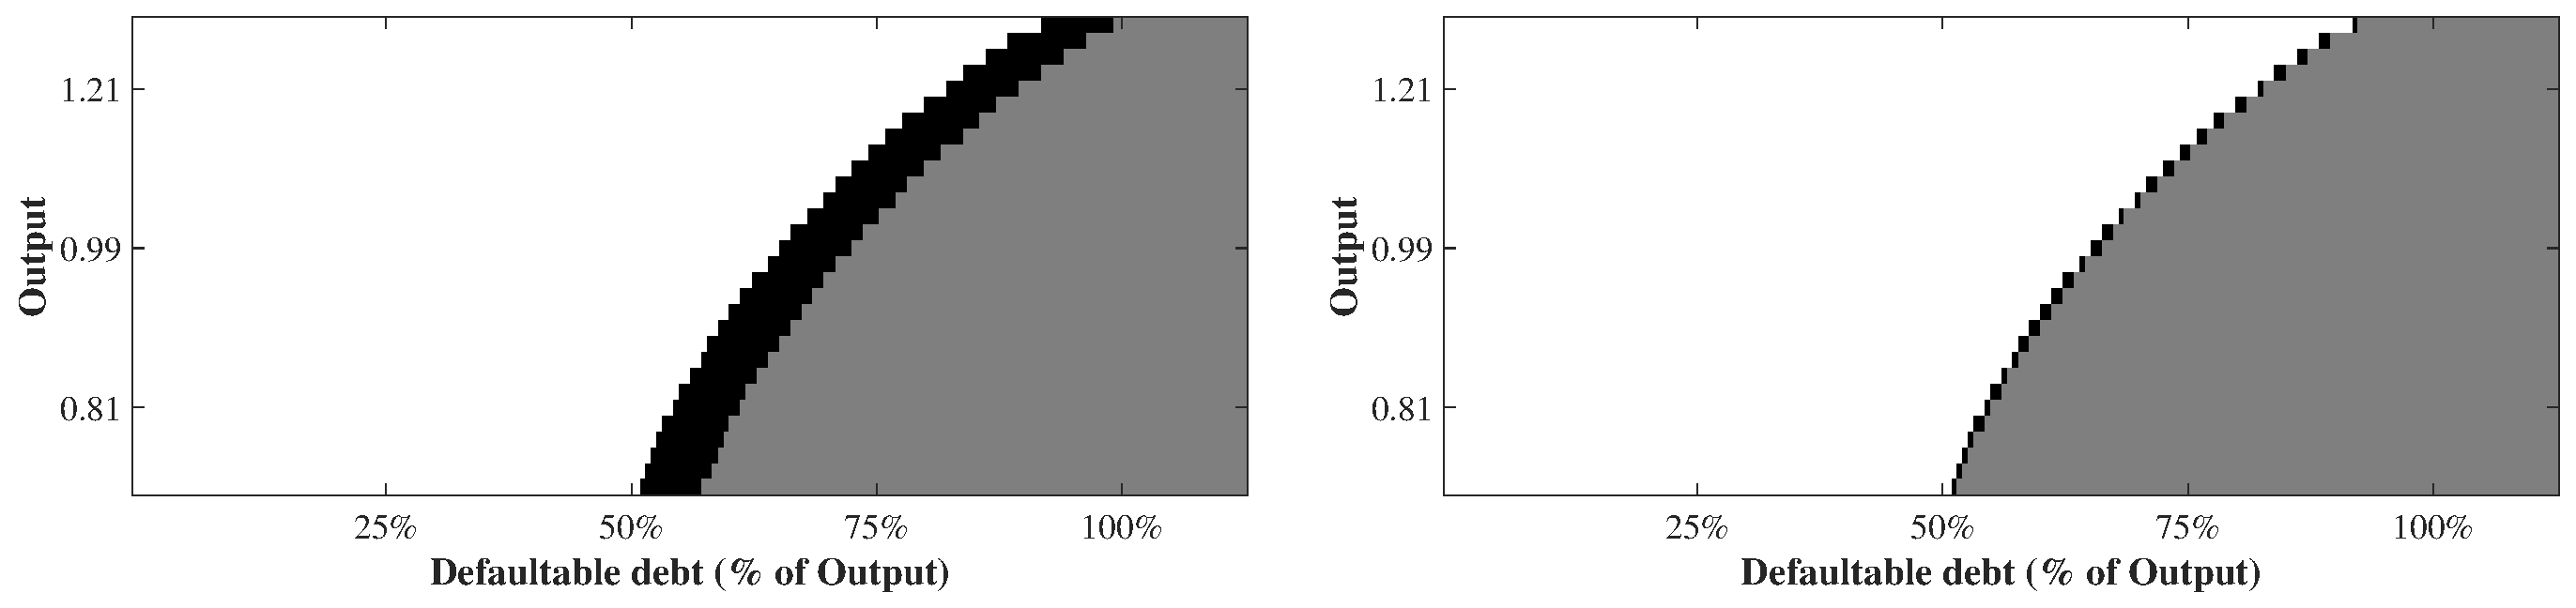
\includegraphics[scale=0.27]{default_decision_baseline.eps}
    }
    \label{fig:default decision}
        \begin{tablenotes}
      \footnotesize
    Figure 3.1 shows the default decision matrix for an economy without (black area) and an economy with Eurobonds (gray area). The left panel displays the decision where for both economies $e = 0$. The right panel shows the default decision where both economies are at their non-defaultable debt limit, $e = 0$ and $e = 0.4$ respectively.
    \end{tablenotes}
\end{figure}
%%%%%%%%%%%%%%%%%%%%%%%%%%%%%%%%%%%%%%%%%%%%%%%%%%%%%%%%%%
The first scenario (Left Panel) we take into consideration is that of two different economies: one without (black area) and one with Eurobonds where $e = 0$ (gray area). The default sets visualized for these circumstances allows us to determine if there are any combinations for defaultable debt $d$ and output $y$ for which a government would default if no Eurobonds are introduced, but would not if they are, and vice versa. As we can see, the gray area is a subset of the black area. This means that there are more combinations $(d,y)$ for which a government would default when Eurobonds are \textit{not} introduced. The reason for this difference in incentives to default can be found in the benefits of having access to non-defaultable debt. When in a state of default, there will be an exclusion period where access to the debt markets, including the one for non-defaultable debt, is limited. Non-defaultable debt can only be rolled over in a state of default and this prospect of limited market access is enough the reduce the combinations $(d,y)$ for which a government would choose to default.\\ 

The second scenario (Right Panel) portrays the default decision where both economies are considered to be at their non-defaultable debt limits, $e = 0$ (black area) and $e = 0.4$ (gray area). Similar to before, the gray area is a subset of the black area, though in a more limited way compared to the first scenario. We can therefore draw the same conclusion as the previous paragraph: default risk decreases after the introduction of Eurobonds because the potential loss of access to both the defaultable and non-defaultable debt market is enough to deter the government to default.\\

\subsubsection{Impulse response functions to introducing Eurobonds}
The second exercise illustrates the short-term effects of Eurobonds. An introduction is simulated by allowing Eurobonds to be issued at time t=0 and each period represents one quarter. Figure \ref{fig:intro} shows the average consumption, defaultable debt, risk premium and non-defaultable debt paths together with their $\pm$ two standard deviations.\\
%%%%%%%%%%%%%%%%%%%%%%%%%%%%%%%%%%%%%%%%%%%%%%%%%%%%%%%%%%
 \begin{figure}[H] 
     \centering
     \caption{\textbf{Eurobond introduction}}
     \vspace{1mm}
      \resizebox{\columnwidth}{!}{%
   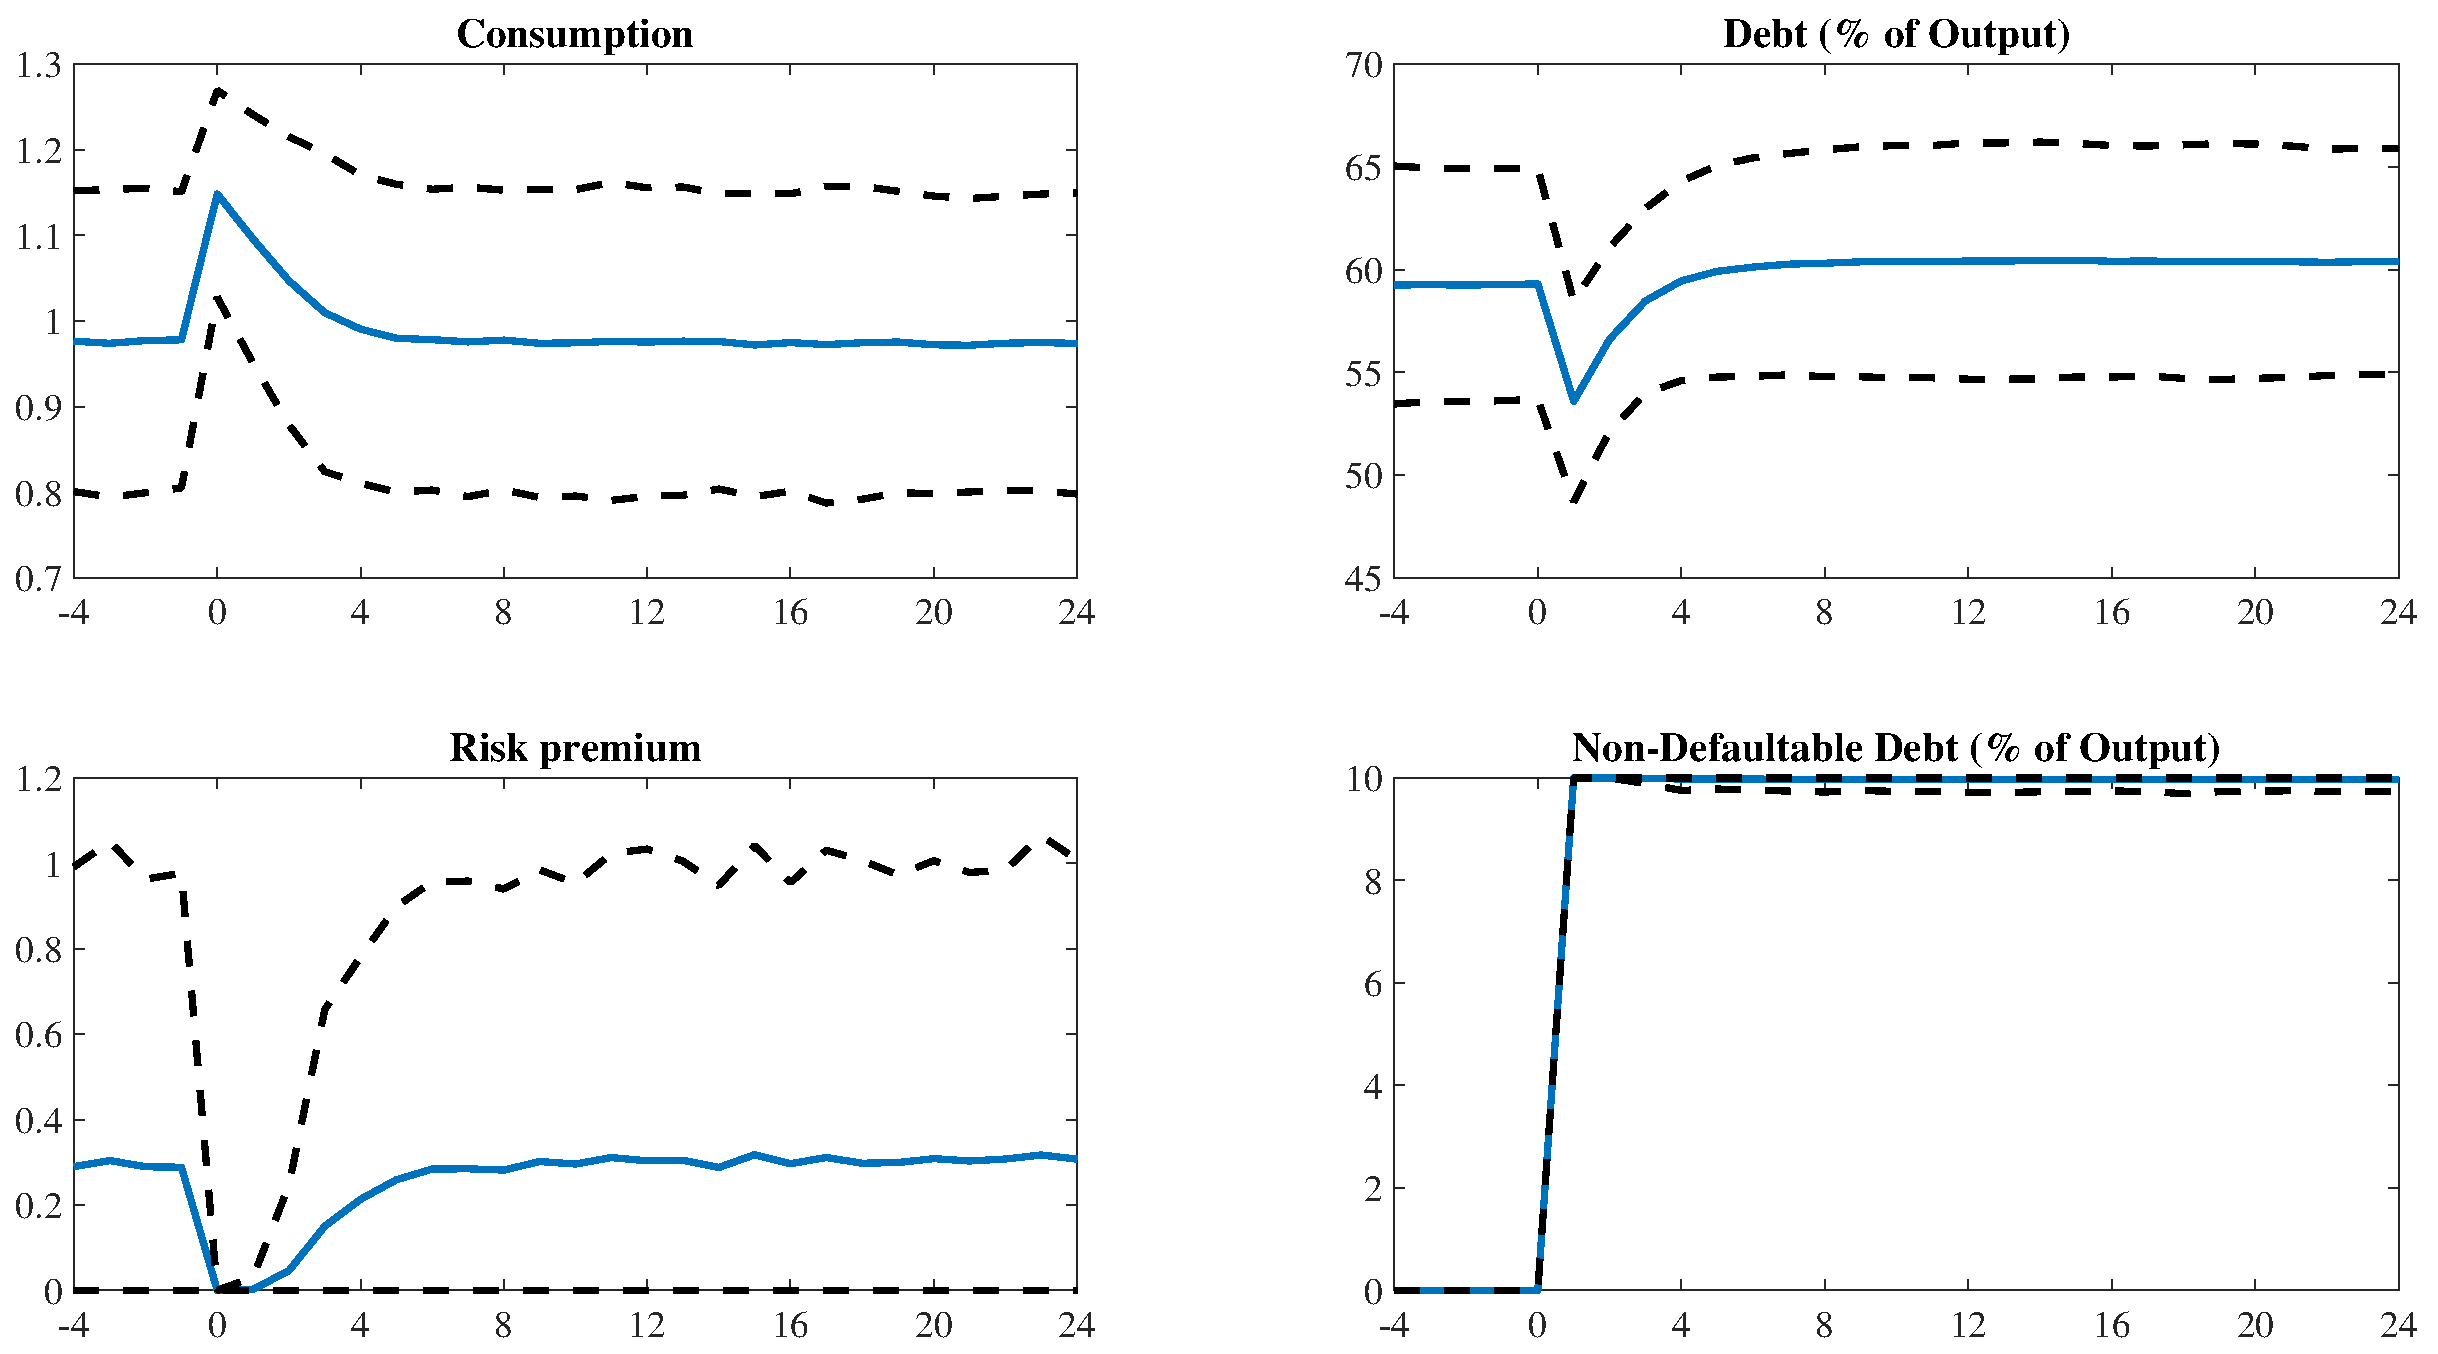
\includegraphics[scale=0.32]{Intro_baseline.eps}
    }\label{fig:intro}
      \begin{tablenotes}
      \footnotesize
      \item Figure 3.2 presents the results of an transitioning from an economy without to an economy with Eurobonds. The introduction occurs at time 0 and the response functions shown are for Consumption (Panel 1), Defaultable debt (Panel 2), the Risk Premium (Panel 3) and Non-defaultable debt (Panel 4). The full line presents the mean response and the dashed lines $\pm$ 2 standard deviations from the mean. Defaultable and non-defaultable debt are reported in \% of annual output.
      \end{tablenotes}
 \end{figure}
%%%%%%%%%%%%%%%%%%%%%%%%%%%%%%%%%%%%%%%%%%%%%%%%%%%%%%%%%%


As seen in the first panel, in the short-term there are welfare gains involved when transitioning from an economy without to one with non-defaultable debt. Consumption increases shortly after the introduction, as the government takes full advantage of the new, cheaper source of funding. On average, the non-defaultable debt limit has already been reached after one quarter. The increase in one form of debt is partially compensated by a decrease in the other. Defaultable debt decreases by roughly 7\%, which is not enough to fully compensate for the increase in its non-defaultable equivalent. This decrease in defaultable debt also lowers the average risk premium and its volatility, implying that the default risk fully disappears at the time of the introduction.\\  

As expected, however, the welfare gains of the introduction are of a short-term nature. After 4 quarters, defaultable debt and the risk premium return to their earlier levels, while non-defaultable debt remains at its limit. As any new debt needs to be repaid, the rise in consumption will also decrease over time. Nevertheless, the extra non-defaultable debt that needs to be repaid has negligible effects on consumption which will return to levels very similar to the ones before the introduction.\\ 

The analysis of the short-term effects is thus complementary to the long-term analysis. While the potential benefits of introducing a new non-defaultable form of debt are of a short-term nature, after a year the economy converges again to an equilibrium with similar defaultable debt levels, yet with a higher non-defaultable debt level. Our form of Eurobonds alone does not impose incentives to control or reduce debt levels in a model with sovereign default. In section 3.3, however, we will consider a credible debt rule which, if committed to, will play the role of a possible additional incentive to compensate for the lack of debt control in the current set-up of the model.\\
\subsection{A typical default episode}
To finalize the discussion of the baseline model, Figure \ref{fig:default_episode} presents the average default episode for an economy without and with Eurobonds. Even though the original purpose of the Eurobonds is not to mitigate default episodes, any significant changes it can have, could be useful to know in the design and policy debate. The simulations are performed for the economy with and without Eurobonds separately and the default occurs at time 0.\\
%%%%%%%%%%%%%%%%%%%%%%%%%%%%%%%%%%%%%%%%%%%%%%%%%%%%%%%%%%
\begin{figure}[H] 
     \centering
     \caption{\textbf{Typical default episode}}
     \vspace{1mm}
      \resizebox{\columnwidth}{!}{%
   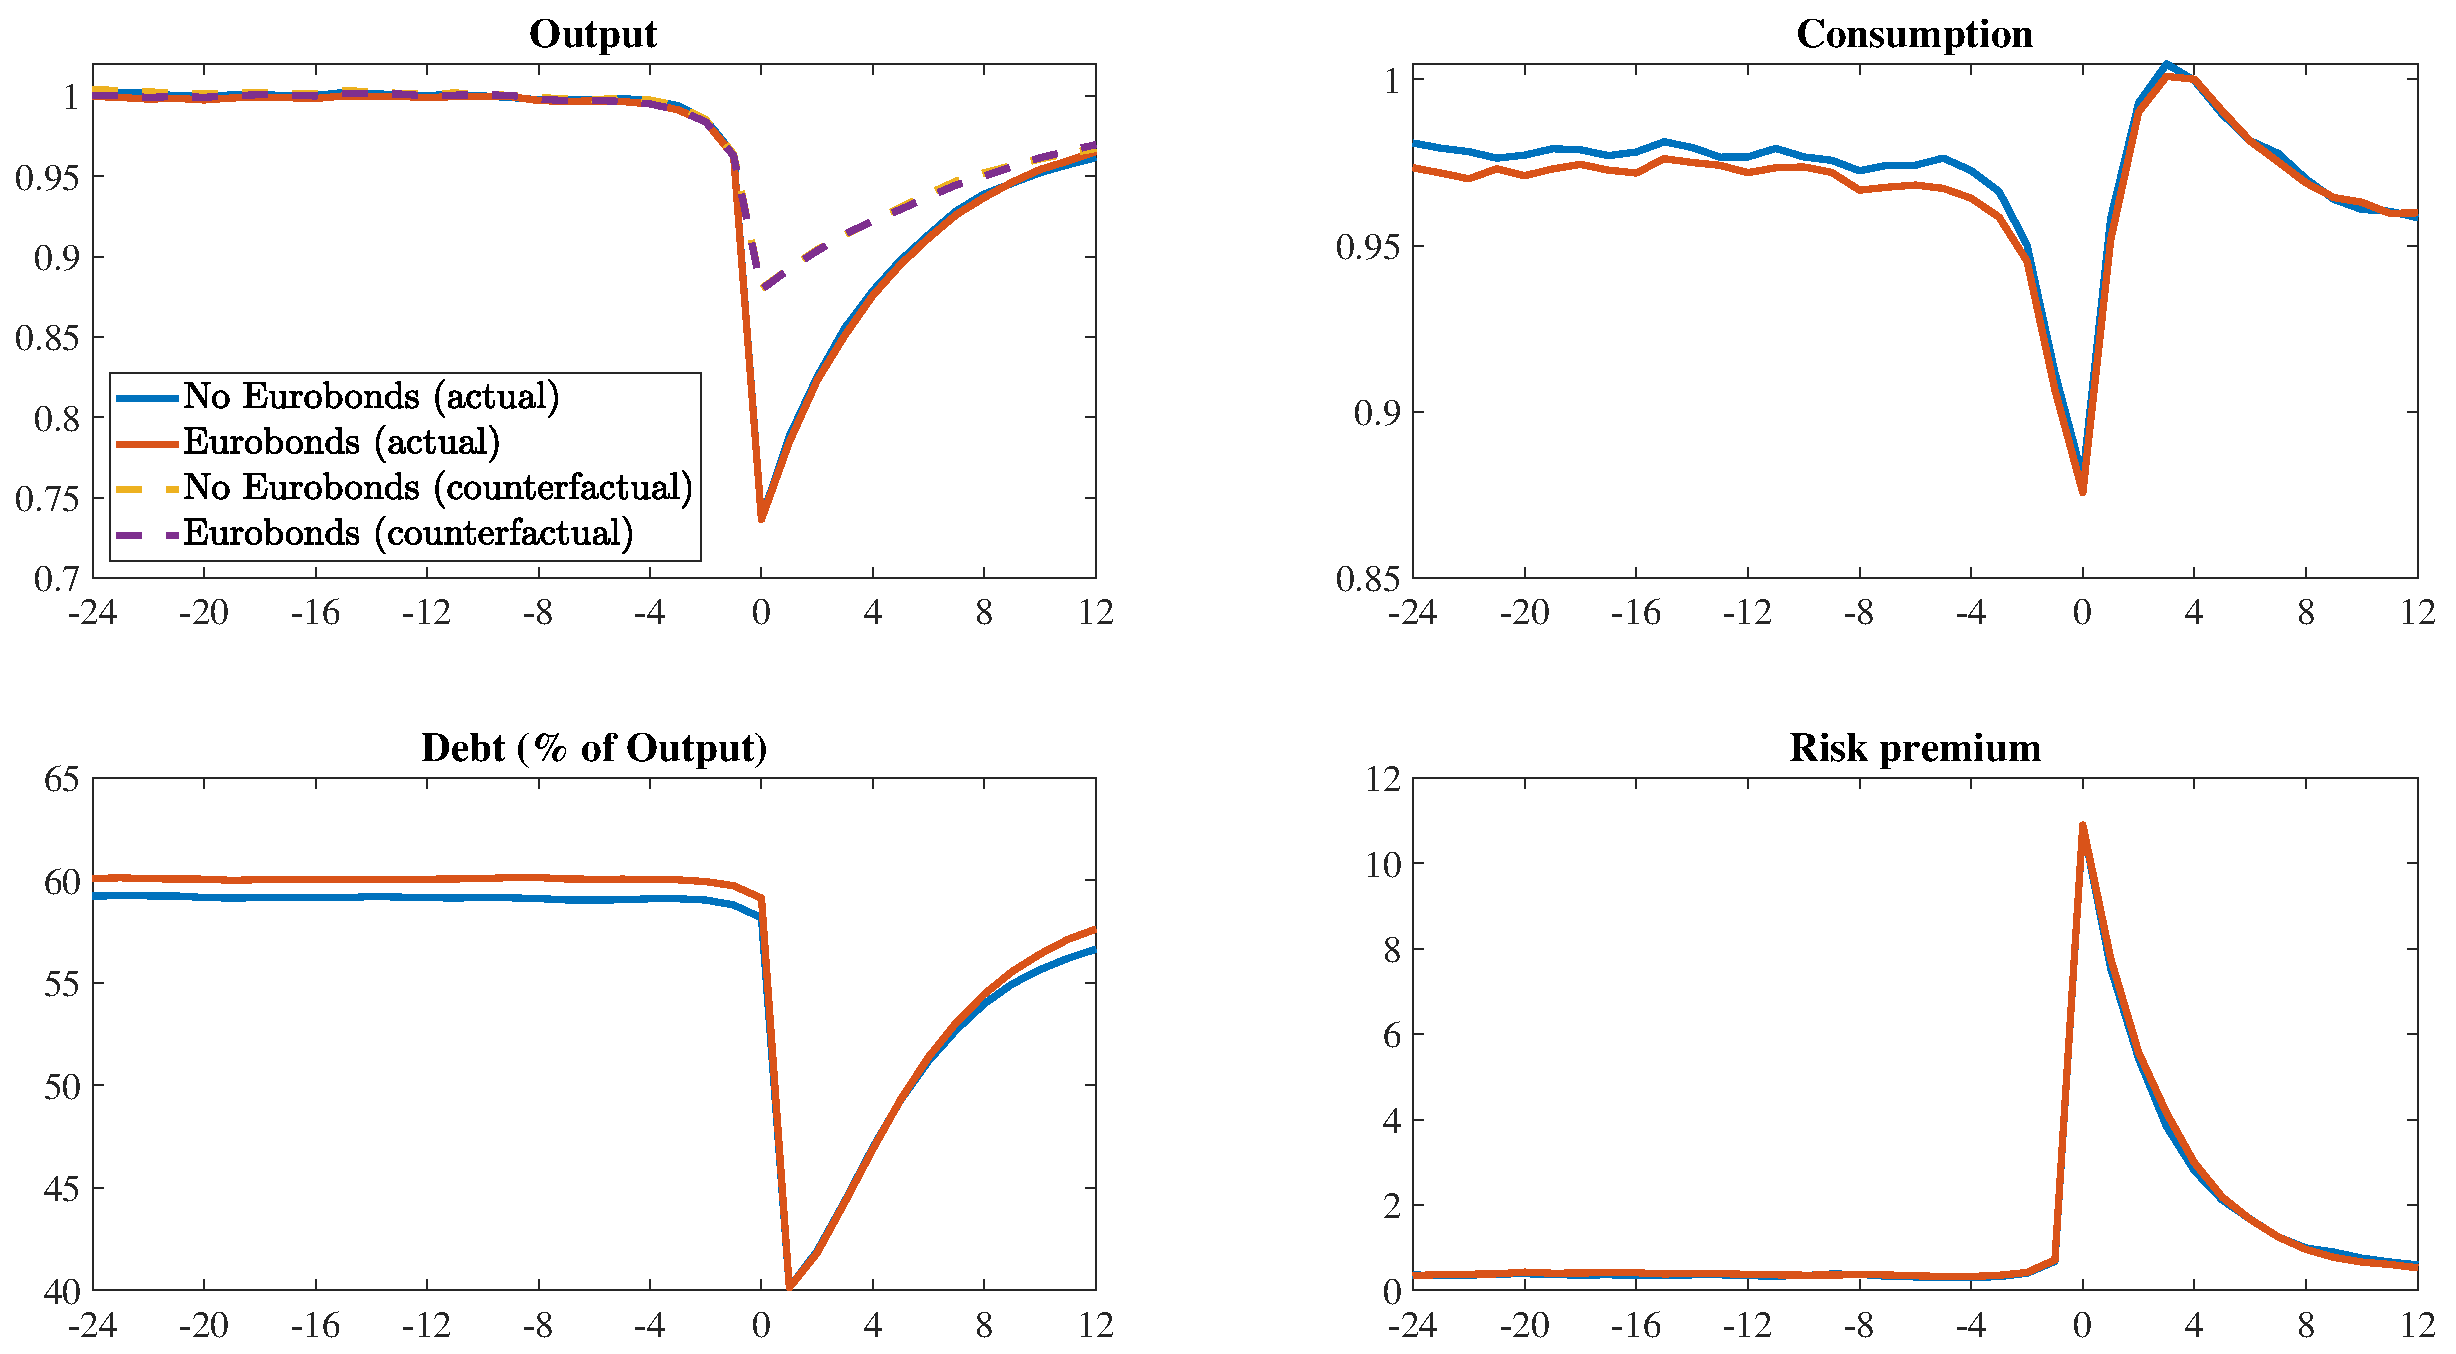
\includegraphics[scale=0.32]{typical_default_baseline.eps}
    }\label{fig:default_episode}
      \begin{tablenotes}
      \footnotesize
      \item Figure 3.4 presents the results of a typical, average default episode for an economy without (blue) and with Eurobonds (red). Average results are presented for Output, Consumption, Defaultable debt in \% of output, the Risk Premium and Non-defaultable debt in \% of output. For panel 1 the full lines present the actual output path and the dashed lines present the output path that would have been followed if no default had occurred (yellow: economy without Eurobonds, purple: economy with Eurobonds). Defaultable debt is reported in \% of annual output.
      \end{tablenotes}
    
 \end{figure}
%%%%%%%%%%%%%%%%%%%%%%%%%%%%%%%%%%%%%%%%%%%%%%%%%%%%%%%%%%
Based on the results from Figure \ref{fig:default_episode} we can make a similar conclusion to the one we made in the long-run analysis: the difference between the economy without and with Eurobonds is negligibly small. For both economies output, consumption and defaultable debt drop significantly after the default occurs, while the risk premium rises. As also shown by the dashed lines, the counterfactual output path that would have been followed had the government not decided to default also drops, though to a lesser extent than the actual path. This gap between the actual and counterfactual paths is created by the income loss $L(y)$ we assumed earlier. Overall, we can conclude our model shows no evidence Eurobonds could mitigate default episodes.\\

\section{The importance of bargaining power}
In the baseline model we assumed that the government has full control when renegotiating its debt level after a default and is committed to a self-imposed renegotiation rule $d_B = \min(d,d_S)$, similar to the model by Hatchondo et al. (2017). In practice this means that, if a default occurs, the government will offer investors a take-it-or-leave-it offer when access to the financial market is regained and investors have no way of influencing the restructured debt level. This assumption, however, may not always hold, as international power generally differs between nations and thus investor may have some influence in certain nations. This section will therefore consider a range of different values for the distribution of bargain power $\alpha$, as done in Yue (2010), and see if changing the power distribution also changes the impact of introducing Eurobonds, either in the long-run, short-run or both.\\

\subsection{Long-run impact of Eurobonds and bargaining power}
Table \ref{tab:alpha} presents the long-run statistics for different distributions of bargaining power. We will consider a range of values for $\alpha \in [0,1]$. For a complete analysis: if $\alpha = 1$ we will also consider the case where a government does not follow a specific restructuring rule and renegotiation is at its full discretion.\\

Based on the results for the different bargain schedules, three main observations can be made. First of all, regardless whether Eurobonds are introduced or not, the defaultable debt level and the default frequency increases for lower values of $\alpha$, while the risk premium and average haircut decreases. Exceptions do occur for $\alpha \in [0,0.25]$ and $\alpha = 0.45$ with Eurobonds. This, however, can be explained by the width of the grid as defaultable debt is at its limit and therefore inadequate to approximate the true solution. Nevertheless, these findings seem to conform to what Yue (2010) and Uribe \& Schmitt-Grohé (2017, p.570-571) concluded. A second observation is that following no restructuring rule ($\alpha = 1$) has a significant impact on how much debt can be supported in equilibrium. With no rule, the average haircut is near 100\% which implies a lot more risk is involved for investors who will adjust their debt pricing accordingly. The third and most important observation is that with the introduction of Eurobonds, defaultable debt levels drastically increase for any $\alpha \neq 1$, though not in a monotonic fashion. In addition, the risk premia are also lower in the economy with Eurobonds, hinting at overall lower risk. The reason as to why this occurs has to do with the influence investors have in renegotiation which we will cover in section 3.2.3.\\
\subsection{Short-run effects of Eurobonds and bargaining power}
Similar to the baseline results, to see the short-run impact of introducing Eurobonds in different bargaining schedules the average impulse response functions of consumption, defaultable debt, the risk premium and non-defaultable debt are visualized in Figure \ref{fig:intro_comp}. We will only consider the cases of $\alpha \in [0.55,1]$ as these give us the most reliable results (cf. Table \ref{tab:alpha}).\\
%%%%%%%%%%%%%%%%%%%%%%%%%%%%%%%%%%%%%%%%%%%%%%%%%%%%%%%%%%
\begin{table}[H]\Large
\setlength{\arrayrulewidth}{0.3mm}
\centering
    \caption{\textbf{Model statistics for different distributions of bargaining power $\alpha$}}
    \label{tab:alpha}
    \vspace{1mm}
   \resizebox{\columnwidth}{!}{%
 \begin{tabular}{lm{2.6cm}cccccc} 
\hline\hline
\textbf {Model}                 &  \textbf {Default frequency}       &$\bm{E(\frac{d}{Y})}$& $\bm{E(\frac{e}{Y})}$&  $\bm{E(r-r^*)}$& $\bm{\sigma(r-r^*)}$ & $\bm{corr(r-r^*,y)}$& $\bm{E(h)}$           \\
\hline\hline
\textit{\underline{Baseline}}  &    &      &     &     &      &  & \\[1ex] 
\textit{\bm{$\alpha = 1 \text{ } \|\text{ } d_B \text{ \textbf{rule} (No Eurobonds)}$}}  & 0.8436    & 59.21     & 0     & 0.2852    & 0.342     & -0.4236   & 30.85 \\[1ex] 
\textit{\bm{$\alpha = 1 \text{ } \|\text{ } d_B \text{ \textbf{rule} (Eurobonds)}$}}  &0.8428     & 60.21     & 9.99  & 0.3034    & 0.3502    &-0.4517    & 32          \\[1ex] 
\textit{\underline{Alternative values for $\alpha$ (No Eurobonds)}}  &    &      &     &     &      &  & \\[1ex] 
\textit{\bm{$\alpha = 0.00 $}}  &  n.a.   &  112.79    &   0 & n.a. & n.a.  &  n.a. & n.a. \\[1ex]                                 
\textit{\bm{$\alpha = 0.25 $}}  &  n.a.   &   112.88   &   0   &    n.a. & n.a.   &  n.a. & n.a.  \\[1ex]                                 
\textit{\bm{$\alpha = 0.45$}}  & 1.9732    &  98.18    &   0   &  0.3613   &  0.4885    & -0.4818  & 13.96 \\[1ex]
\textit{\bm{$\alpha = 0.55$}}  & 1.714    & 79.26  & 0  &  0.395    &  0.5307   &   -0.4928   &   19.29  \\[1ex]
\textit{\bm{$\alpha = 0.65$}} &1.5656 &  63.36   &  0    & 0.4866     & 0.6651    &  -0.4898    &   26.63  \\[1ex]
\textit{\bm{$\alpha = 0.75$}}  &  1.2836   &   49.52   &  0    &  0.5434   &    0.7248  & -0.489  & 36.84 \\[1ex]
\textit{\bm{$\alpha = 1.00 \text{ } \| \text{\textbf{ no }} d_B \text{\textbf{ rule}}$}}  & 0.7912    & 22.21     & 0     & 0.8671    & 1.0413     & -0.4862   & 99.99\\[1ex] 
\textit{\underline{Alternative values for $\alpha$ (Eurobonds)}}  &    &      &     &     &      &  & \\[1ex]
\textit{\bm{$\alpha = 0.00$}}  &  n.a. & 112.83  & 10.03     &    n.a. & n.a.   &   n.a. & n.a.  \\[1ex]  
\textit{\bm{$\alpha = 0.25$}}  &   n.a. & 112.77  &10.02    &      n.a. & n.a.     & n.a. & n.a. \\[1ex] 
\textit{\bm{$\alpha = 0.45$}}  & 0.3468 & 112.53  & 10.02  &  0.0481  &  0.1630 &  -0.5256 & 9.66  \\[1ex] 
\textit{\bm{$\alpha = 0.55$}}  &  1.7072 &  95.75  &  9.96   & 0.3239 &   0.4354 &  -0.4997 & 15.33  \\[1ex]
\textit{\bm{$\alpha = 0.65$}}  &  1.5576  & 75.29 &   9.98  &  0.4103  &  0.5535 &  -0.4933 &  22.04\\[1ex]
\textit{\bm{$\alpha = 0.75$}}  &   1.2880  & 57.54 &9.92  &  0.4678   & 0.6245  & -0.4772  &  31.78\\[1ex]
\textit{\bm{$\alpha = 1.00 \text{ } \| \text{\textbf{ no }} d_B \text{\textbf{ rule}}$}}  & 0.7300 &  23.63  &  9.90    &0.7479   & 0.8979  & -0.4553 & 97.47          \\[1ex]     
\hline\hline
\end{tabular}}
    \begin{tablenotes}
      \footnotesize
      \item Model statistics are calculated under the condition a country finds itself in good standing. The default frequency is reported on an annual basis. The symbols E, $\sigma$ and corr represent the average, standard deviation and correlation. Average defaultable $E(\frac{d}{Y})$ and non-defaultable debt $E(\frac{e}{Y})$ are reported in \% of annual output $Y = 4y$. The Risk Premium and haircut are presented as $r-r^*$ and $h$, respectively. The special case $\alpha = 1$ is calculated once with (baseline) and once without the special rule for $d_B$ (alternative).
    \end{tablenotes}
\end{table}
%%%%%%%%%%%%%%%%%%%%%%%%%%%%%%%%%%%%%%%%%%%%%%%%%%%%%%%%%%


While we find that for all values of $\alpha$ there are welfare gains of introducing Eurobonds, the intensity of these gains varies between the different economies. The economies where investors have more influence in the restructuring process ($\alpha = \{0.55,0.65,0.75\}$) lead to a significantly higher increase in consumption compared to the economy where they have no influence. This can partially be explained by the lower initial buyback or decrease in defaultable debt for lower values of $\alpha$. This combined with the relatively higher decrease in risk premia and increase in non-defaultable debt leads to a higher and longer increase in consumption as consumption returns to its original level only after 8 quarters compared to 4 quarters in the baseline model.  Nonetheless, the most notable difference seems once more to occur in medium- to long-run convergence of the defaultable debt level. For all economies with $\alpha \neq 1$ the defaultable debt level converges to a higher level than before the introduction, implying the influence of investors is non-trivial.\\
%%%%%%%%%%%%%%%%%%%%%%%%%%%%%%%%%%%%%%%%%%%%%%%%%%%%%%%%%%
 \begin{figure}[H]
\caption{\textbf{Introducing the Eurobond in different bargaining schedules}}
    \centering
    \vspace{1mm}
     \resizebox{\columnwidth}{!}{%
   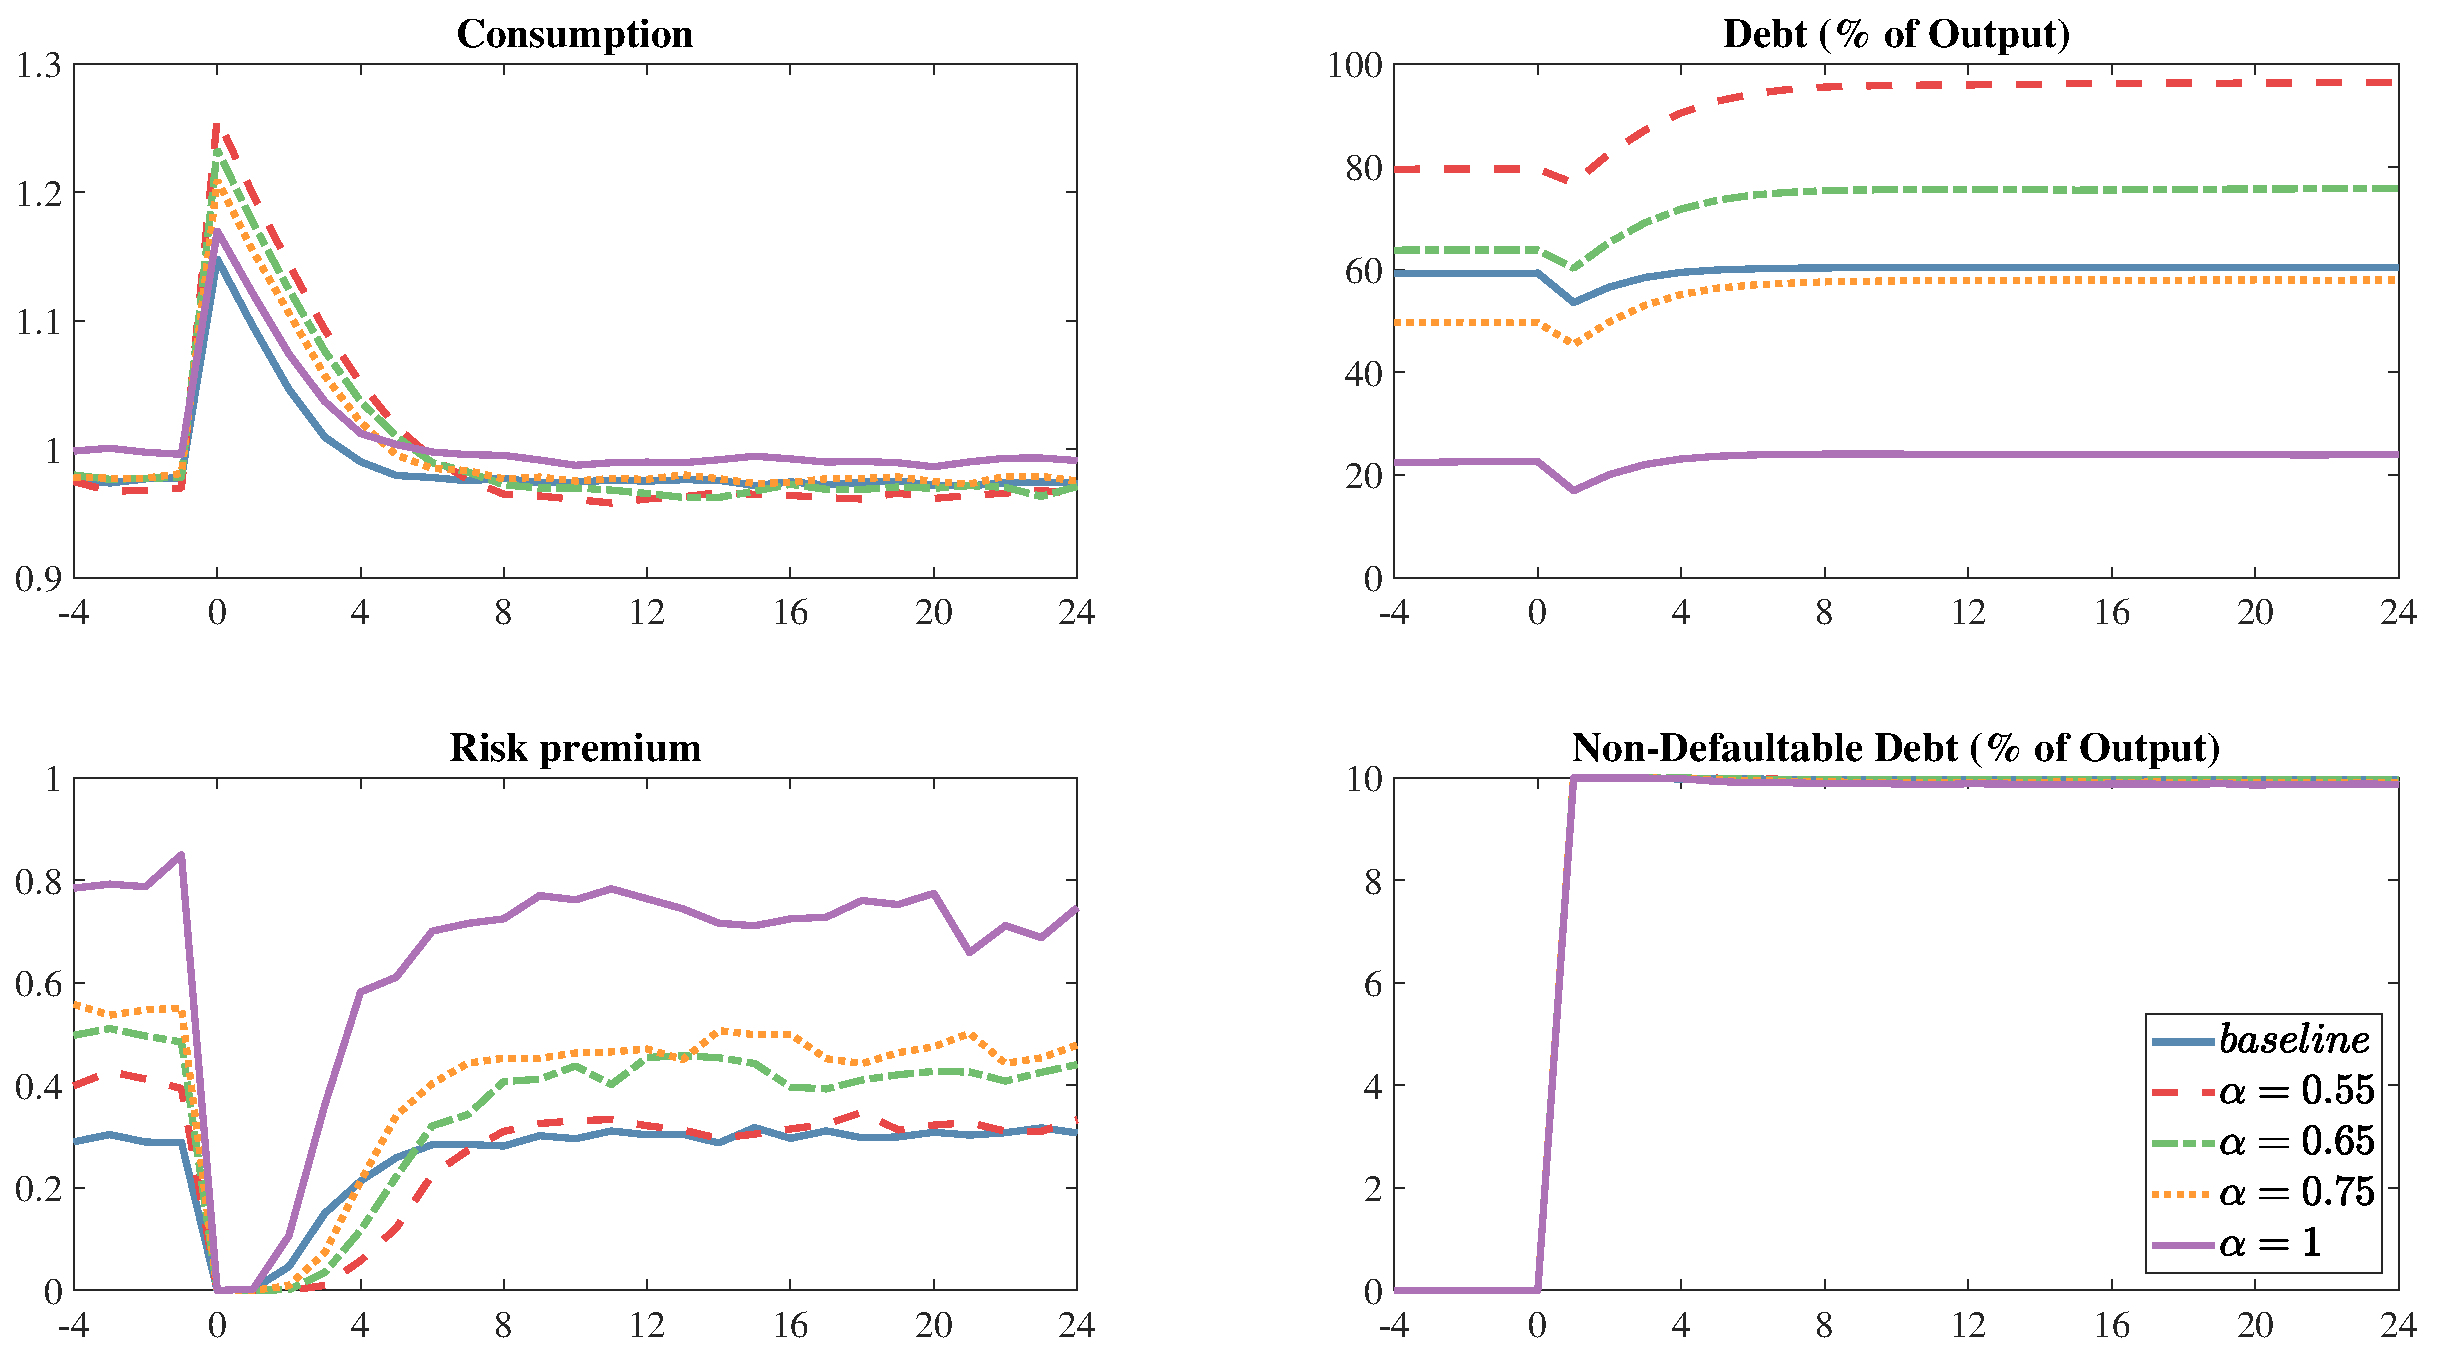
\includegraphics[scale=0.28]{Intro_comp.eps}
    }
    \label{fig:intro_comp}
        \begin{tablenotes}
      \footnotesize
   Figure 3.4 presents the results of transitioning from an economy without to an economy with Eurobonds for the baseline model and different values for $\alpha$. The introduction occurs at time 0 and the average response functions are shown for Consumption (Panel 1), Defaultable debt (Panel 2), the Risk Premium (Panel 3) and Non-defaultable debt (Panel 4). Defaultable and non-defaultable debt are reported in \% of annual output.
    \end{tablenotes}
\end{figure}
%%%%%%%%%%%%%%%%%%%%%%%%%%%%%%%%%%%%%%%%%%%%%%%%%%%%%%%%%%
\subsection{The influence of investors after the introduction of Eurobonds}
Both the long-run and short-run analysis show that the bargain power distribution has a significant impact on the long-run debt level when Eurobonds are introduced. This impact is most apparent for $\alpha \in [0.55,0.75]$. To explain these differences, we will distinguish two phases in which the role of investors affect the debt incentive structure: the renegotiation phase and a "Price \& Debt adjustment" phase.\\

 In the renegotiation phase, there is a distinction between $\alpha = 1$ and $\alpha \neq 1$. If $\alpha = 1$ the government has full control and its optimal strategy will not change, regardless if it has access to Eurobonds or not. If $\alpha \neq 1$, however, investors will be involved in the renegotiation process and a compromise needs to be found between the two interest groups. Recall that the surplus of the investors is determined by $q_B(d_B,e,y)d_B$ and that the default risk decreases for some combinations of $(d,y)$ as shown by Figure \ref{fig:default decision} (complemented by Figures A.1-A.4 in Appendix A). This suggests that, as soon as Eurobonds are introduced, default risk decreases for certain combinations of $(d,y)$ which results in a higher price $q$ and $q_B$ for debt in this region. Because of this higher price, creditors will also gain a larger surplus if they readjust their bargain position, particularly for those combinations of $(d,y)$ that were considered to be risky before, yet not anymore. With the readjustment in the bargain position of investors and an unchanged strategy for the government, the result of the renegotiation is a higher recovery rate $\frac{d_B(y)}{d}$ after default, which explains the lower haircut after the introduction of Eurobonds.\\ 
 
 This renegotiation phase is then followed by a "Price \& Debt adjustment" phase. As the recovery rate increases after the introduction of Eurobonds, investors will once more readjust the pricing of debt contracts. After all, the recovery rate is part of the price equations \eqref{ZP not default} and \eqref{ZP default}. With a higher recovery rate investors will lose less if a default occurs, therefore prices of debt will go up as there is less risk involved. From the government's point of view higher prices for debt imply lower costs of borrowing, making borrowing more attractive. The government will thus take advantage of this reduction in costs and seek to increase its borrowing level.\\
 
What results out of the two phases is what we observe both in Table \ref{tab:alpha} and Figure \ref{fig:intro_comp}: the frequency of defaults stays relatively the same after the introduction of Eurobonds, while debt levels, both defaultable and non-defaultable, increase more if investors can exert more influence on the renegotiation process. The policy implication that follows from this extension is that disregarding the balance of power can affect the overall evaluation of Eurobonds. Nations with different bargain power may experience different changes in incentive structures. Without any additional debt control incentives debt levels can rise significantly, especially for those nations where investors are able to influence the restructuring process.\\

\section{Potential benefit of a credible debt rule}
As a last addition to our analysis we will simulate the effects of introducing Eurobonds together with a credible debt rule. Considering that Eurobonds do not incentivise governments to reduce debt, additional fiscal rules may need to be imposed to guarantee compliance with the fiscal framework of the European Union. As argued by Hatchondo et al. (2017) introducing Eurobonds could also potentially help in financing this transition to specific fiscal rules or targets. The question then remains: do Eurobonds still provide benefits if introduced with additional fiscal rules?\\

Figure \ref{fig:intro_debtrule} shows the result of introducing Eurobonds together with a debt rule. In combination with the announcement of Eurobonds, the government announces that a new debt rule of a defaultable debt-to-GDP ratio of 50\% will be imposed. We will not go into detail on how it is implemented and we simply assume it to be a rule to which the government is able to commit. The limit of defaultable debt to 50\% is chosen such that it reduces all risk of default and is conform to the Maastricht criteria of 60\% debt-to-GDP when summed up with the non-defaultable debt limit (European Commission, 2019).\\

Despite the limitation on defaultable debt, introducing Eurobonds still delivers benefits to welfare in the short-run. All economies\footnote{Note that $\alpha = 1$ without a $d_B$ rule is left out of Figure \ref{fig:intro_debtrule}, since introducing a debt rule of 50\% would have no effect on this parameterisation of the model.} experience an increase in consumption and a reduction in defaultable debt and risk premia. Unlike the scenario without a debt rule, however, the increase in consumption is more short-lived for the economies with lower $\alpha$'s. Nonetheless, the commitment to the debt rule reduces defaultable debt in the long-run to the extent that all default risk disappears and borrowing is done at the risk-free rate.\\
%%%%%%%%%%%%%%%%%%%%%%%%%%%%%%%%%%%%%%%%%%%%%%%%%%%%%%%%%%
 \begin{figure}[H]
\caption{\textbf{Introducing the Eurobond in different bargaining schedules together with a debt rule}}
    \centering
    \vspace{1mm}
     \resizebox{\columnwidth}{!}{%
   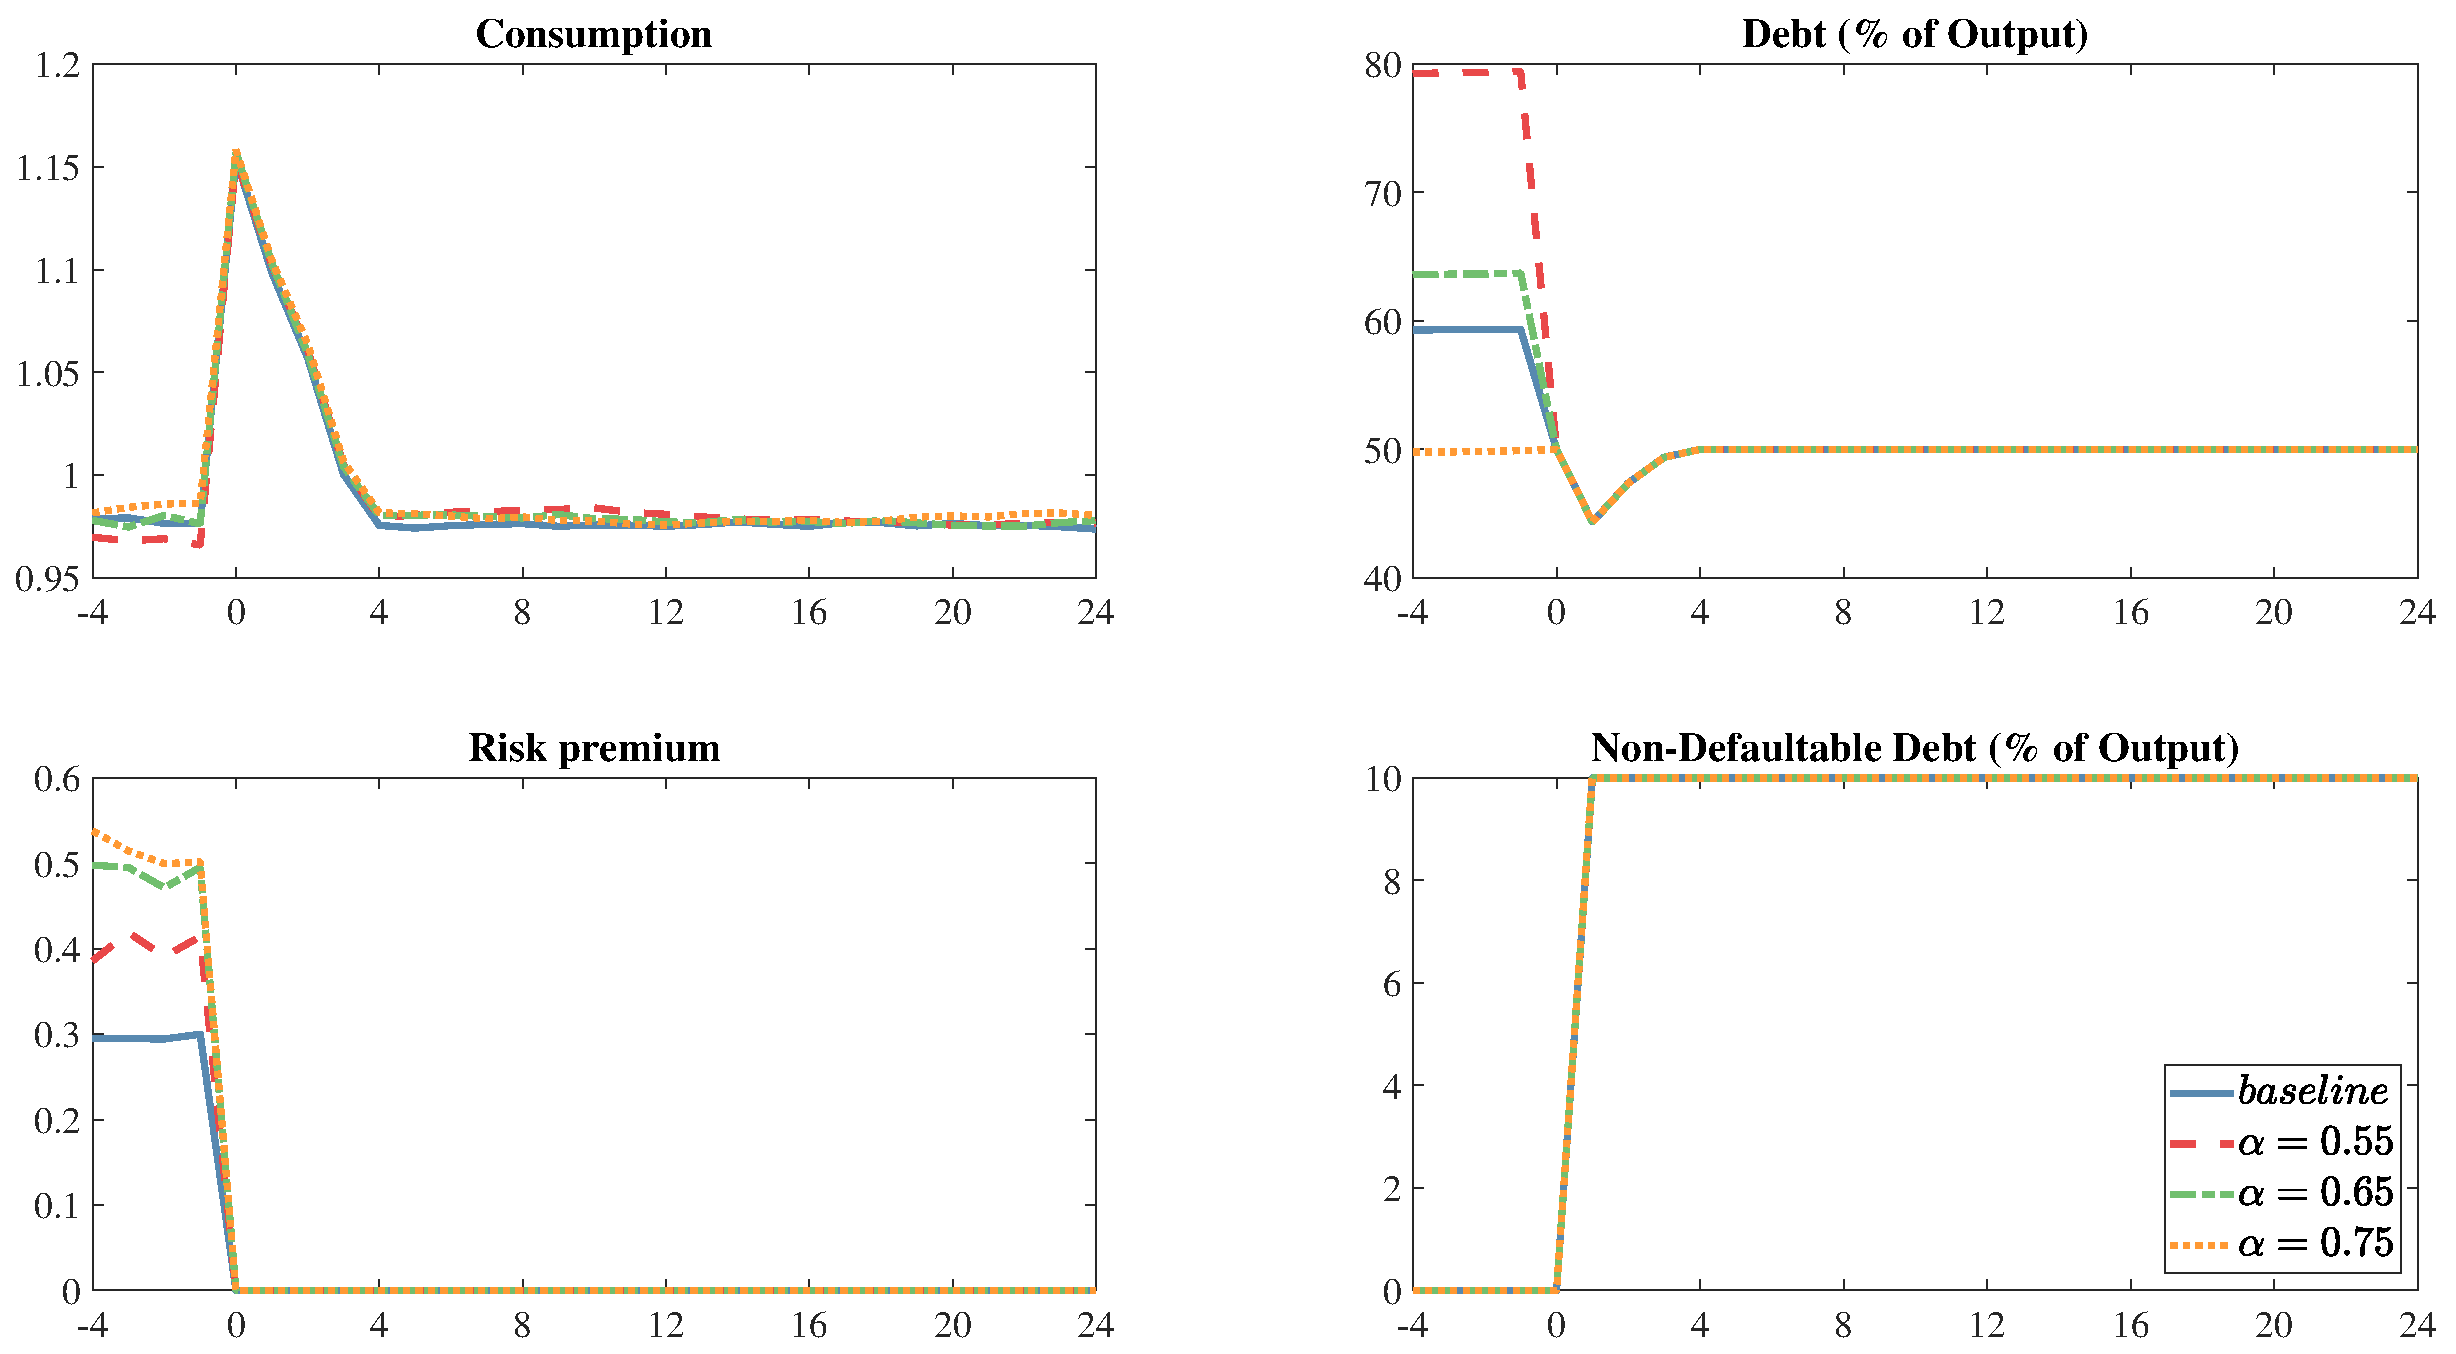
\includegraphics[scale=0.28]{Intro_debtrule.eps}
    }
    \label{fig:intro_debtrule}
        \begin{tablenotes}
      \footnotesize
   Figure 3.5 presents the results of transitioning from an economy without to an economy with Eurobonds for the baseline model and different values for $\alpha$ in addition to a debt rule. The introduction occurs at time 0 and the average response functions shown are for Consumption (Panel 1), Defaultable debt (Panel 2), the Risk Premium (Panel 3) and Non-defaultable debt (Panel 4). Defaultable and non-defaultable debt are reported in \% of annual output. To ensure compatibility of the two calibrated models and their policy functions, the number of grid points for Defaultable Debt nd is lowered to 100 in the economy with the debt rule.
    \end{tablenotes}
\end{figure}
%%%%%%%%%%%%%%%%%%%%%%%%%%%%%%%%%%%%%%%%%%%%%%%%%%%%%%%%%%
\section{Robustness of the model}
As a final step in our analysis, we will perform a robustness check of the baseline model. Four specific tests to the robustness of our results will be considered: the sensitivity to alternatives of the exclusion duration $\theta$, the sensitivity to the non-defaultable debt limit, the sensitivity to the grid specification and, lastly, the possible occurrence of multiple equilibria.\\
\subsection{Sensitivity to the duration of the exclusion period}
In the baseline model it is assumed that once a default occurs, access to financial markets is regained within the year (3.5 quarters for $\theta = 0.282$). The use of this calibrated value conforms to estimates by Gelos et al. (2004) and is used by several papers in the sovereign default literature (e.g. Hatchondo et al., 2017; Önder \& Sunel,  2020). However, Gelos et al.'s estimates are based on a data-set of developing economies and a revision of their earlier work re-estimates an average exclusion of 2.9 years based on data from the 1990s (Gelos, Sahay \& Sandleris, 2011). As our model is calibrated to a European economy, we consider a more prudent stance and test the sensitivity of the results to different probabilities of reentry $\theta$.\\
\clearpage
To account for some possible uncertainty we will re-calibrate the baseline model to a lower and higher value for $\theta$ and see how this affects the results. The higher value is a fictional value of 0.5 which implies a shorter, average reentry within 2 quarters. The lower value we calibrate to the findings of Guscina, Malik \& Papaioannou (2017) who estimate an average exclusion period of 19 months ($\theta = 0.210$) between the period of 2010-2015 for a data-set of both developing and developed countries.\\

Table \ref{tab:theta} shows the results for the different calibrations of $\theta$. Conform to the expectations, a lower $\theta$ corresponds to a lower default frequency. A longer exclusion period makes defaulting less attractive as access to financial markets is lost for a longer period of time. With these lower default incentives, investors will price bonds higher which in turn allows for a higher debt level. The opposite interactions can be observed when $\theta$ is higher. That being said, different values of $\theta$ do not seem to alter our conclusion on Eurobonds from the baseline model. Both economies behave similarly in the long-run and any differences are negligibly small.\\
%%%%%%%%%%%%%%%%%%%%%%%%%%%%%%%%%%%%%%%%%%%%%%%%%%%%%%%%%%
\begin{table}[H]\Large
\setlength{\arrayrulewidth}{0.3mm}
\centering
    \caption{\textbf{Model statistics for different reentry probabilities $\theta$}}
    \label{tab:theta}
    \vspace{1mm}
   \resizebox{\columnwidth}{!}{%
 \begin{tabular}{lm{2.1cm}cccccc} 
\hline\hline
\textbf {Model}                 &  \textbf {Default frequency}       &$\bm{E(\frac{d}{Y})}$& $\bm{E(\frac{e}{Y})}$&  $\bm{E(r-r^*)}$& $\bm{\sigma(r-r^*)}$ & $\bm{corr(r-r^*,y)}$& $\bm{E(h)}$           \\
\hline\hline
\textit{\underline{Baseline}}  &    &      &     &     &      &  & \\[1ex] 
\textit{\bm{$\theta = 0.282 \text{ (No Eurobonds)}$}}  & 0.8436    & 59.21     & 0     & 0.2852    & 0.342     & -0.4236   & 30.85 \\[1ex] 
\textit{\bm{$\theta = 0.282 \text{ (Eurobonds)}$}}   &0.8428     & 60.21     & 9.99  & 0.3034    & 0.3502    &-0.4517    & 32          \\[1ex]   
\textit{\underline{Alternative values for $\theta$}}  &    &      &     &     &      &  & \\[1ex] 
\textit{\bm{$\theta = 0.210 \text{ (No Eurobonds)}$}}  &  0.6512  & 66.33  &      0  &  0.2847  &  0.3759  & -0.4170 & 38.36\\[1ex] 
\textit{\bm{$\theta = 0.210 \text{ (Eurobonds)}$}}  &  0.6904  & 68.15  &  9.52 &   0.3165 &   0.3720 &  -0.4234 & 40.23        \\[1ex]
\textit{\bm{$\theta = 0.500 \text{ (No Eurobonds)}$}}  & 1.1480  & 50.59  &      0 &   0.2528  &  0.2508  & -0.3567  & 19.56\\[1ex] 
\textit{\bm{$\theta = 0.500 \text{ (Eurobonds)}$}}  &    1.0828 &  51.15  & 9.99  &  0.2504  &  0.2366  & -0.4359   &     20.27   \\[1ex]     \hline\hline
\end{tabular}}    
\begin{tablenotes}
      \footnotesize
      \item Model statistics are calculated under the condition a country finds itself in good standing. The default frequency is reported on an annual basis. The symbols E, $\sigma$ and corr represent the average, standard deviation and correlation. Average defaultable $E(\frac{d}{Y})$ and non-defaultable debt $E(\frac{e}{Y})$ are reported in \% of annual output $Y = 4y$. The risk premium and haircut are presented as $r-r^*$ and $h$, respectively.
    \end{tablenotes}
\end{table}
%%%%%%%%%%%%%%%%%%%%%%%%%%%%%%%%%%%%%%%%%%%%%%%%%%%%%%%%%%
\subsection{Sensitivity to the non-defaultable debt limit}
Similar to the analysis performed by Hatchondo et al. (2017) we assumed that the non-defaultable debt limit was set at 10\% of GDP. Setting this limit makes our analysis comparable to Philippon \& Hellwig's Eurobill proposal (2011). Other proposals, for example the Blue-Red bond proposal by Delpla \& Von Weizsäcker (2010) or the Redemption Pact (Doluca et al., 2012), suggest a larger percentage of debt to be mutualised. The model can be easily adjusted to account for these larger Eurobond limits by increasing the upper limit $\bar{e}_R$. We will perform a smaller adjustment of up to 20\% and a larger change of up to 60\% to test the sensitivity of our results. A drawback of extending the upper limit, however, is that by doing so we also increase the coarseness of the grid if we do not also increase the number of grid points. The discussion on the importance of the grid specification is left for section 3.4.3.\\ 
%%%%%%%%%%%%%%%%%%%%%%%%%%%%%%%%%%%%%%%%%%%%%%%%%%%%%%%%%%
\begin{table}[H]\large
\setlength{\arrayrulewidth}{0.3mm}
\centering
    \caption{\textbf{Sensitivity of results to the non-defaultable debt limit}}
    \label{tab:non-defaultable debt limit}
    \vspace{1mm}
   \resizebox{\columnwidth}{!}{%
 \begin{tabular}{lm{2.5cm}cccccc} 
\hline\hline
\textbf {Model}                 &  \textbf {Default frequency}       &$\bm{E(\frac{d}{Y})}$& $\bm{E(\frac{e}{Y})}$&  $\bm{E(r-r^*)}$& $\bm{\sigma(r-r^*)}$ & $\bm{corr(r-r^*,y)}$& $\bm{E(h)}$           \\
\hline\hline
\textit{\bm{$\bar{e}_R = 0.4$}}     &0.8428     & 60.21     & 9.99  & 0.3034    & 0.3502    &-0.4517    & 32          \\[1ex]    
\textit{\bm{$\bar{e}_R = 0.8$}}     &0.7412&   60.89 & 20.04 &   0.2745  &  0.3256  & -0.3953 & 32.95\\[1ex]
\textit{\bm{$\bar{e}_R = 2.4$}}     &0.7692 &  64.11 &  60.16  &  0.3047 &   0.3549  & -0.4157 & 36.29 \\[1ex]      
\hline\hline             
\end{tabular}}
    \begin{tablenotes}
      \footnotesize
      \item Model statistics are calculated under the condition a country finds itself in good standing. The default frequency is reported on an annual basis. The symbols E, $\sigma$ and corr represent the average, standard deviation and correlation. Average defaultable $E(\frac{d}{Y})$ and non-defaultable debt $E(\frac{e}{Y})$ are reported in \% of annual output $Y = 4y$. The risk premium and haircut are presented as $r-r^*$ and $h$, respectively.
    \end{tablenotes}
\end{table}
%%%%%%%%%%%%%%%%%%%%%%%%%%%%%%%%%%%%%%%%%%%%%%%%%%%%%%%%%%
Table \ref{tab:non-defaultable debt limit} shows that altering the non-defaultable debt limit has no large impact on the model performance, other than increasing the average non-defaultable debt-to-GDP ratio. Both economies with $\bar{e}_R = 0.8$ and $\bar{e}_R = 2.4$ will stay at their Eurobond limit in the long-run and there are no incentives to decrease defaultable debt, similar to the results of the baseline model.\\
\subsection{Sensitivity to the grid specification}
Hatchondo, Martinez \& Sapriza (2010) caution in their paper on numerical solution methods of sovereign default models that using Discrete State Space approaches with an insufficient amount of grid points can lead to spurious interest rate movements and unreliable results. Uribe \& Schmitt-Grohé (2017, p.530-533) also support this critique by showing that increasing or decreasing the endowment grid can alter the results of the model. To test for possible misspecification, we consider 9 alternative grids for our model. In our analysis, however, we limited the number of possible elements of a grid to 120.000 as working with larger grids often led to memory issues or extremely long computation times in \texttt{Matlab}.\\

Table \ref{tab:grid} lists the results for our different grid specifications. To study the sensitivity we perform four categories of alterations: i) a variation of different non-defaultable debt points $ne$, ii) a variation of different defaultable debt points $nd$, iii) a variation of both defaultable and non-defaultable points $(nd,ne)$ and iv) a variation of output points $ny$.\\

The results of Table \ref{tab:grid} show that while the predictions do not deviate much of one another, some caution is warranted. Estimates for the default frequency range from 0.704 to 0.9292, which corresponds to a default every 142 to 108 years. Furthermore, even as defaultable debt stays around 60\%, its non-defaultable counterpart seems to be sensitive to changes in both the defaultable and non-defaultable debt grid. Both for a lower amount of grid points $nd$ and higher amount for $ne$ does the average debt ratio for Eurobonds decrease, from 9.99\% in the baseline to 7.8\% in the grid (30,20,200). This implies that our earlier finding that non-defaultable debt is almost always at its limit may be a result of our chosen grid and thus not entirely accurate for all grid approximations.\\
%%%%%%%%%%%%%%%%%%%%%%%%%%%%%%%%%%%%%%%%%%%%%%%%%%%%%%%%%%
\begin{table}[H]\Large
\setlength{\arrayrulewidth}{0.3mm}
\centering
    \caption{\textbf{Model statistics for different grid specifications}}
    \label{tab:grid}
    \vspace{1mm}
   \resizebox{\columnwidth}{!}{%
 \begin{tabular}{lm{2.6cm}cccccc} 
\hline\hline
\textbf {Grid size}                 &  \textbf {Default frequency}       &$\bm{E(\frac{d}{Y})}$& $\bm{E(\frac{e}{Y})}$&  $\bm{E(r-r^*)}$& $\bm{\sigma(r-r^*)}$ & $\bm{corr(r-r^*,y)}$& $\bm{E(h)}$           \\
\hline\hline
\textit{\underline{Baseline}}  &    &      &     &     &      &  & \\[1ex]                                 
\textit{\bm{$(30,200,20)$}}  & 0.8428     & 60.21     & 9.99  & 0.3034    & 0.3502    &-0.4517    & 32          \\[1ex]   
\textit{\underline{Varying ne}}  &    &      &     &     &      &  & \\[1ex]                                 
\textit{\bm{$(30,200,10)$}} & 0.9292 &  59.93 &  10.02  &  0.3265  &  0.4148  & -0.3658& 31.93\\[1ex]                                 
\textit{\bm{$(30,200,5)$}}  & 0.7820   & 60.49     & 9.80    & 0.2972    & 0.3558     & -0.4198 & 32.56\\[1ex]
\textit{\underline{Varying nd}}  &    &      &     &     &      &  & \\[1ex]                                 
\textit{\bm{$(30,100,20)$}} & 0.7040 &  60.38&   9.19   & 0.2671  &  0.2935  & -0.4281  & 33.31\\[1ex] 
\textit{\bm{$(30,50,20)$}}  &   0.7140  & 60.10  &  8.95 &   0.2834 &   0.3292 &  -0.4086  & 34.04\\[1ex]  
\textit{\bm{$(30,25,20)$}}  & 0.7520  & 63.47  &  8.31 &   0.2884  &  0.3562 & -0.3583 & 32.68\\[1ex]
\textit{\underline{Varying (nd,ne)}}  &    &      &     &     &      &  & \\[1ex]                                 
\textit{\bm{$(30,75,50)$}}  &    0.7696  & 60.44 &  9.47&   0.2864  &  0.3330  & -0.4164&33.39 \\[1ex]                                 
\textit{\bm{$(30,20,200)$}}  &   0.7540  & 63.76&   7.82  & 0.2785  &  0.3264  & -0.4070  &33.90 \\[1ex]      
\textit{\underline{Varying ny}}  &    &      &     &     &      &  & \\[1ex]                                 
\textit{\bm{$(60,100,20)$}}  &   0.8544  & 59.42  &  9.97   & 0.3097  &  0.3601 &  -0.4101  & 31.71\\[1ex]                                 
\textit{\bm{$(200,20,20)$}}  &  0.7228  & 62.63 &   7.94 &   0.2742 &   0.2698  & -0.4821 & 32.65\\[1ex]                                 
\hline\hline
\end{tabular}}
    \begin{tablenotes}
      \footnotesize
      \item Model statistics are calculated under the condition a country finds itself in good standing. The default frequency is reported on an annual basis. The symbols E, $\sigma$ and corr represent the average, standard deviation and correlation. Average defaultable $E(\frac{d}{Y})$ and non-defaultable debt $E(\frac{e}{Y})$ are reported in \% of annual output $Y = 4y$. The risk premium and haircut are presented as $r-r^*$ and $h$, respectively.
    \end{tablenotes}
\end{table}
%%%%%%%%%%%%%%%%%%%%%%%%%%%%%%%%%%%%%%%%%%%%%%%%%%%%%%%%%%
The issue that arises when we decide on the correct grid specification is the trade-off between computational burden and precision in a DSS approach. Due to this trade-off and our limitation on the possible number of grid points, we are limited in our testing of the grid validity. Because of this, some caution about the results is advised and possible further testing should be performed. The possibility of using interpolation methods as suggested by Hatchondo et al. (2010) could also be considered as an alternative to solving the model more efficiently and in improving the accuracy.\\

\subsection{Possibility of multiple equilibria}
The last robustness check we will perform is a check for multiple equilibria. Within the literature, several papers have touched on this subject and have argued in favor of (e.g. Ayres, et al, 2018) or against the possibility of equilibria (e.g. Auclert \& Rognlie, 2016). Given that there is some degree of uncertainty and given that Aguiar \& Amadar (2019) show that the set-up we use for the sovereign default model is not a contraction mapping, we will take a careful approach and explicitly test whether the model is subject to it or not.\\
\clearpage
We will follow Önder's (2016) prescription for a practical implementation of Auclert \& Rognlie's suggestion to test multiple equilibria. The idea behind it is to start our value function iteration process from two distinct starting points: a "good" equilibrium and a "bad" equilibrium. If both starting points lead to very similar model solutions, we should have no problem with multiple equilibria. For each starting point, we attribute the following starting values to the default decision $\hat{p}$ and price functions $q$ and $q_B$:
\begin{itemize}
    \item \textbf{"Good" Equilibrium:} $\hat{p} = 0$ \& $q = q_B = \frac{1}{1+r^*}$
    \item \textbf{"Bad" Equilibrium:} $ \hat{p} = 1$ \& $q = q_B = 0$
\end{itemize}
The "good" equilibrium embodies the starting position where no defaults would occur and borrowing is done at the risk-free rate. The "bad" equilibrium is the opposite and default would occur for every combination of $(d,e,y)$.\\    
%%%%%%%%%%%%%%%%%%%%%%%%%%%%%%%%%%%%%%%%%%%%%%%%%%%%%%%%%%
\begin{table}[H]\Large
\setlength{\arrayrulewidth}{0.3mm}
\centering
   \caption{\textbf{Multiplicity of Equilibria}}
    \label{tab:equilibria}
    \vspace{1mm}
   \resizebox{\columnwidth}{!}{%
 \begin{tabular}{lm{2.5cm}cccccc} 
\hline\hline
\textbf {Model}                 &  \textbf {Default frequency}       &$\bm{E(\frac{d}{Y})}$& $\bm{E(\frac{e}{Y})}$&  $\bm{E(r-r^*)}$& $\bm{\sigma(r-r^*)}$ & $\bm{corr(r-r^*,y)}$& $\bm{E(h)}$           \\
\hline\hline
\textit{\underline{No Eurobonds}}  &    &      &     &     &      &  & \\[1ex]
\textit{\textbf{"Good" Equilibrium}}      & 0.8436    & 59.21     & 0     & 0.2852    & 0.342     & -0.4236   & 30.85\\[1ex]
\textit{\textbf{"Bad" Equilibrium}}     & 0.8240  & 59.40    &     0  &  0.2894  &  0.340  & -0.3983  &  31.26        \\[1ex]
\textit{\underline{Eurobonds}}  &    &      &     &     &      &  & \\[1ex] 
\textit{\textbf{"Good" Equilibrium}}     &0.8428     & 60.21     & 9.99  & 0.3034    & 0.3502    &-0.4517    & 32          \\[1ex]
\textit{\textbf{"Bad" Equilibrium}}  &  0.8192 &  60.24 &    9.98  &  0.2982  &  0.3392  & -0.4176  &  32.18        \\[1ex]
\hline\hline
\end{tabular}}
    \begin{tablenotes}
      \footnotesize
      \item Model statistics are calculated under the condition a country finds itself in good standing. The default frequency is reported on an annual basis. The symbols E, $\sigma$ and corr represent the average, standard deviation and correlation. Average defaultable $E(\frac{d}{Y})$ and non-defaultable debt $E(\frac{e}{Y})$ are reported in \% of annual output $Y = 4y$. The risk premium and haircut are presented as $r-r^*$ and $h$, respectively.
    \end{tablenotes}
\end{table}
%%%%%%%%%%%%%%%%%%%%%%%%%%%%%%%%%%%%%%%%%%%%%%%%%%%%%%%%%%
Once more, we solve the baseline model with the different starting points and as a first exercise we present the long-run statistics in Table \ref{tab:equilibria}. For both starting positions the model leads to similar long-run statistics and shows no indication of significant deviations. Defaultable debt levels remain around 60\% and differences in the risk premia and default frequencies are negligibly small.\\

A second exercise we perform to test the possibility of multiple equilibria is by visualizing the differences in policy functions $\hat{d}, \hat{d}_B, \hat{p}$ and price function $q$. The results for the economy without and with Eurobonds are presented by Figure 3.6 and Figure 3.7, respectively.\\

For the economy without Eurobonds there seems to be some divergent outcomes in policy functions between the "good" and "bad" equilibria. While some of these differences remain small for the policy function $\hat{d}_B$, there are spikes in deviations between outcomes for the policy functions $\hat{d}$, $\hat{p}$ and price function $q$. These deviations seem to occur in the region of low output levels and mid-to-high defaultable debt levels. The economy with Eurobonds for $e = 0$ shows similar signs of deviations, though to a smaller extent.\\

These findings are inconsistent with what Önder (2016) finds as he finds much smaller deviations between the outcomes for one period debt. One possible explanation for the different conclusion is that Önder uses interpolation methods to solve his model, while this dissertation uses a DSS approach. Overall, we can conclude that while for the larger part of the grid there is no evidence of multiplicity, large deviations in certain regions should keep us cautious about the validity of our model and results.\\
%%%%%%%%%%%%%%%%%%%%%%%%%%%%%%%%%%%%%%%%%%%%%%%%%%%%%%%%%%
 \begin{figure}[H] \label{fig:mult no eurobond}
 \caption{\textbf{Differences in Policy and Price functions (No Eurobonds)}}
 \resizebox{\columnwidth}{!}{%
   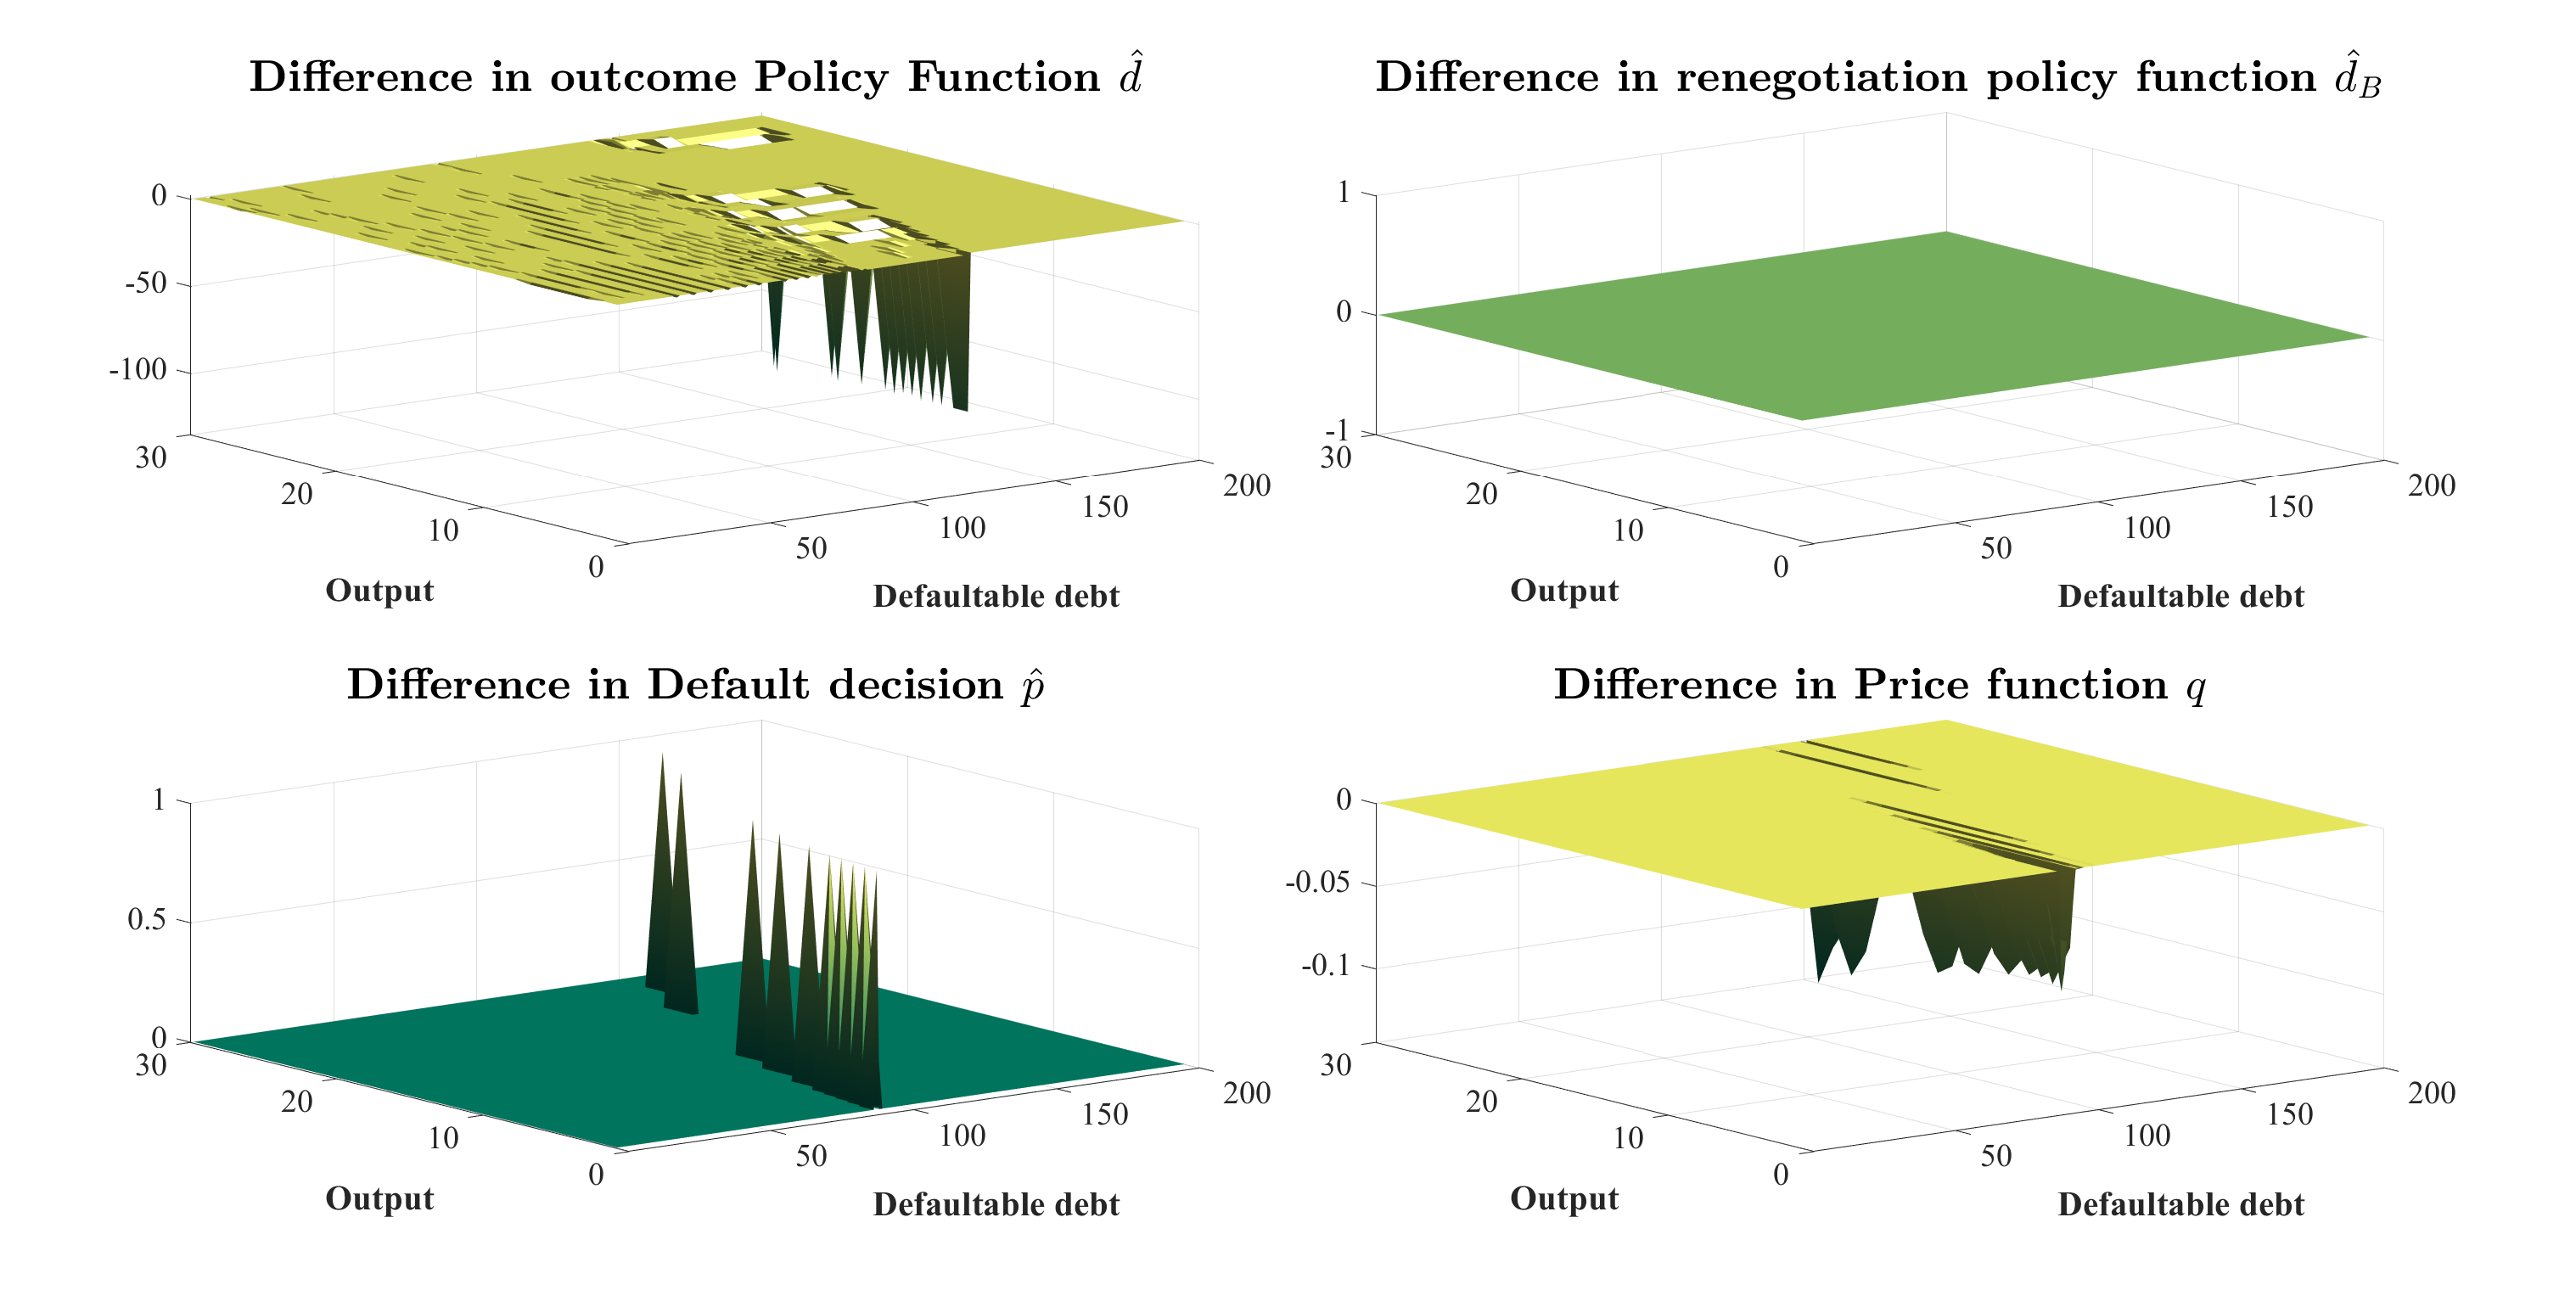
\includegraphics[scale=0.32]{FigureMult_NO.eps}
   }
       \begin{tablenotes}
      \footnotesize
      \item Figure 3.6 presents the differences in policy functions $\hat{d}$, $\hat{d}_B$, default decision $\hat{p}$ and price function $q$ between the "good" equilibrium and "bad" equilibrium starting position. 
    \end{tablenotes}
\end{figure}
%%%%%%%%%%%%%%%%%%%%%%%%%%%%%%%%%%%%%%%%%%%%%%%%%%%%%%%%%%
%%%%%%%%%%%%%%%%%%%%%%%%%%%%%%%%%%%%%%%%%%%%%%%%%%%%%%%%%%
\begin{figure}[H] \label{fig:mult eurobond}
 \caption{\textbf{Differences in Policy and Price functions (Eurobonds)}}
 \resizebox{\columnwidth}{!}{%
   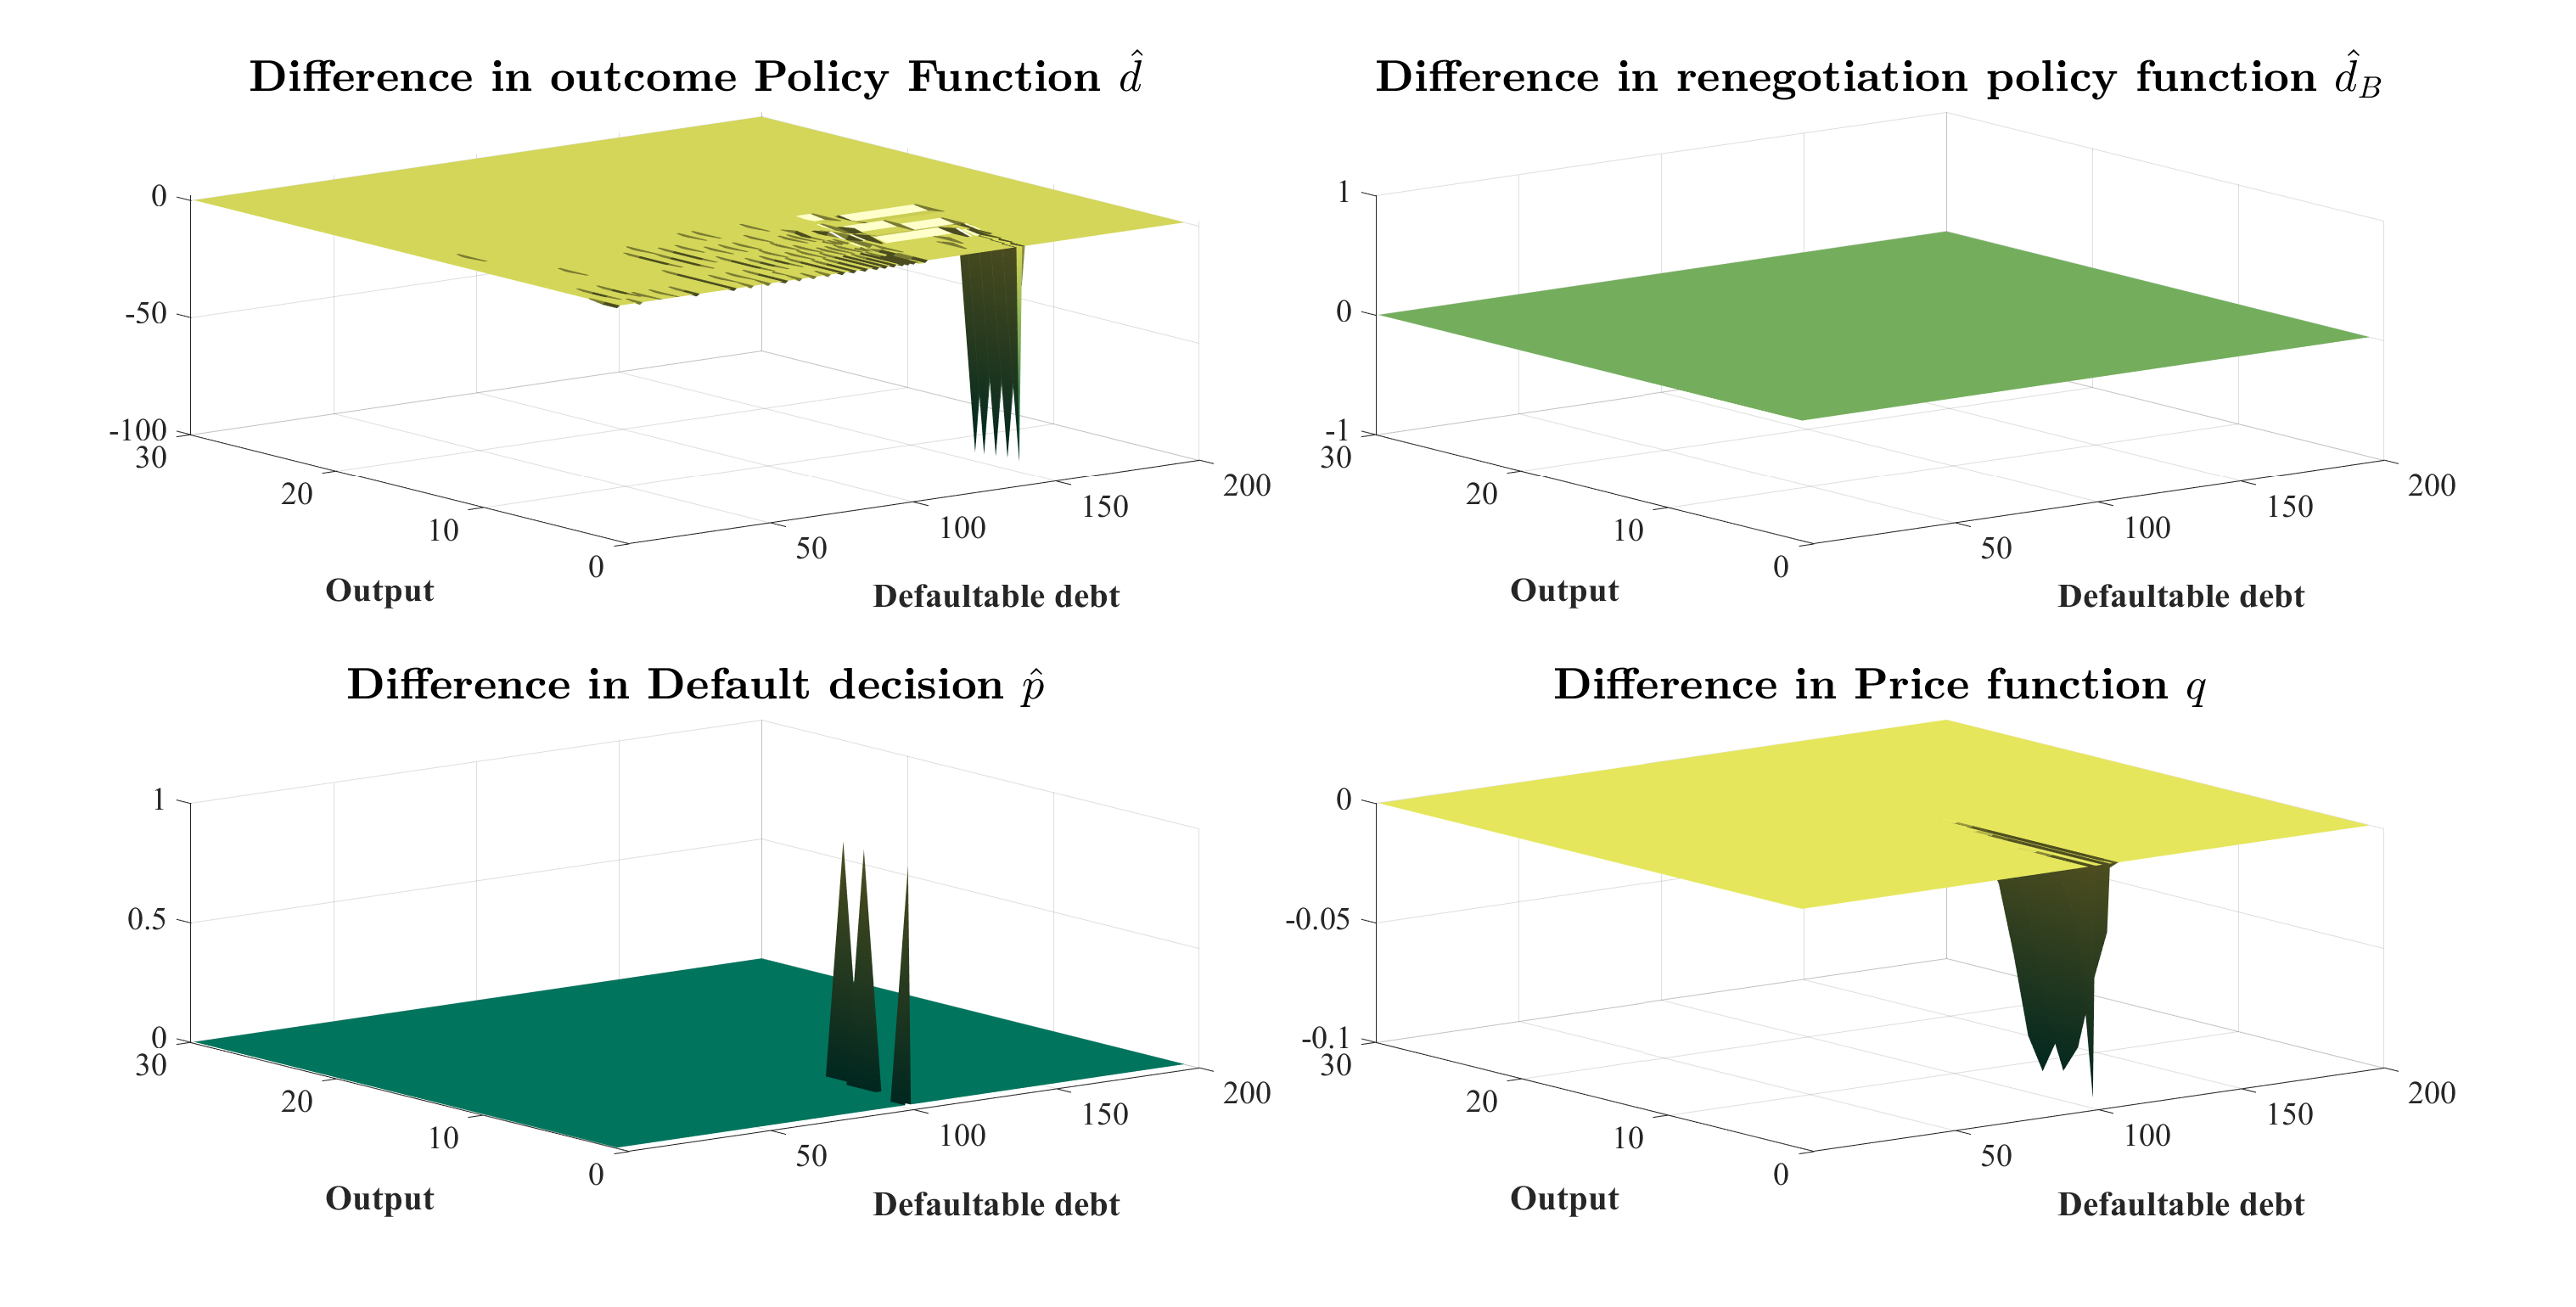
\includegraphics[scale=0.32]{FigureMult_YES.eps}
   }
       \begin{tablenotes}
      \footnotesize
      \item Figure 3.7 presents the differences in policy functions $\hat{d}$, $\hat{d}_B$, default decision $\hat{p}$ and price function $q$ between the "good" equilibrium and "bad" equilibrium starting position. Differences are calculated for each grid point. Only the grid points where $e = 0$ are shown.
    \end{tablenotes}
\end{figure}
%%%%%%%%%%%%%%%%%%%%%%%%%%%%%%%%%%%%%%%%%%%%%%%%%%%%%%%%%%
\pagestyle{headings}
\chapter*{Conclusion}\addcontentsline{toc}{chapter}{Conclusion}
The aim of this dissertation was to study the impact of Eurobonds in a setting of sovereign default following the set-up of Hatchondo et al. (2017). The main contribution is the simultaneous analysis of an introduction of a non-defaultable asset and a debt restructuring process based on a Nash-Bargain game. If the introduction of a Eurobond is considered in isolation, the welfare gains are situated in the short-run, while in the long-run defaultable debt levels and risk premia converge to their original level. When a bargain game is introduced à la Yue (2010), the long-run aspect changes. Investors will have an incentive to re-evaluate their bargain position and will demand a higher recovery rate after a default. The higher recovery rate in turn leads to price and debt adjustments by both investors and the government, finally resulting in a higher overall debt level. In our model, Eurobonds alone do not provide incentives to reduce debt levels. This supports the argument that if the purpose of Eurobonds is to strengthen fiscal discipline, they should be introduced with additional fiscal rules.\\

However, our results do warrant several remarks which can be used as foundation for future research. First of all, a first deviation we made from Hatchondo et al. (2017) is to only consider the case of one period defaultable debt. If long-term debt is introduced, interest rates are no longer only dependent on next period's default risk, but also on subsequent periods. In their paper, they find that the introduction of Eurobonds does reduce the risk premium, however not completely to zero. Long-term debt could therefore lead to a more nuanced conclusion about the distribution of bargaining power, since the decrease in default risk is what triggers investors to re-evaluate their bargain strategy. For a complete analysis, the case of long-term debt should also be considered.\\

A second deviation from the original work is made by choosing a Discrete State Space approach to solve the model. In the original paper, Hatchondo et al. used linear interpolation for endowment levels and spline interpolation for defaultable debt levels. The advantage of using interpolation methods is the potential gains in efficiency and accuracy as discussed in Hatchondo et al. (2010). The analysis from the robustness of the grid specification and multiple equilibria gives us reason to be cautious about the results. Therefore, further research should be performed to test the validity of our model and interpolation methods could be a powerful tool to do so.\\

A final remark concerns the introduction of a credible debt rule. We did not cover how this rule could be implemented and different rules might have different results. A complementary issue is that the assumption of an exogenous output process rules out the influence that government borrowing might have on growth or the business cycle. Further research in this area can prove fruitful in our understanding of Eurobonds.\\ 

%Bibiografie
\clearpage
\pagenumbering{Roman}
\setcounter{page}{5}
%you have to add the bibliography items in mijnbibliografie.bib. Most editors offer a menu for this. Also, in google scholar (settings, advanced) you can turn on @get bibtex citation@, this gives you a text to copy in the bibfile.
\chapter*{Bibliography}
\addcontentsline{toc}{chapter}{Bibliography}
\textbf{Aguiar, M., \& Amador, M. (2019).} A contraction for sovereign debt models. Journal of Economic Theory, 183, 842–875. \url{https://doi.org/10.1016/j.jet.2019.08.005}\\

\textbf{Aguiar, M., \& Gopinath, G. (2006).} Defaultable debt, interest rates and the current account. Journal of International Economics, 69(1), 64–83.\url{https://doi.org/10.1016/j.jinteco.2005.05.005}\\

\textbf{Alfaro, L., \& Kanczuk, F. (2007).} Optimal Reserve Management and Sovereign Debt (SSRN Scholarly Paper ID 996077). Social Science Research Network. \url{https://doi.org/10.2139/ssrn.996077}\\

\textbf{Arellano, C. (2008).} Default Risk and Income Fluctuations in Emerging Economies. American Economic Review, 98(3), 690–712. \url{https://doi.org/10.1257/aer.98.3.690}\\

\textbf{Arellano, C., \& Ramanarayanan, A. (2012).} Default and the Maturity Structure in Sovereign Bonds. Journal of Political Economy, 120(2), 187–232. \url{https://doi.org/10.1086/666589}\\

\textbf{Auclert, A., \& Rognlie, M. (2016).} Unique equilibrium in the Eaton–Gersovitz model of sovereign debt. Journal of Monetary Economics, 84, 134–146. \url{https://doi.org/10.1016/j.jmoneco.2016.10.013}\\

\textbf{Ayres, J., Navarro, G., Nicolini, J. P., \& Teles, P. (2018).} Sovereign default: The role of expectations. Journal of Economic Theory, 175, 803–812. \url{https://doi.org/10.1016/j.jet.2018.02.006}\\

\textbf{Bellman, R. E. (1954).} The Theory of Dynamic Programming. RAND Corporation. \url{https://www.rand.org/pubs/papers/P550.html}\\

\textbf{Bénassy-Quéré, A., Boot, A., Fatás, A., Fratzscher, M., Fuest, C., Giavazzi, F., Marimon, R., Martin, P., Pisani-Ferry, J., Reichlin, L., Schoenmaker, D., Teles, P., \& Mauro, B. W. di. (2020a).} A proposal for a Covid Credit Line. VoxEU.Org. \url{https://voxeu.org/article/proposal-covid-credit-line}\\
\clearpage
\textbf{Bénassy-Quéré, A., Corsetti, G., Fatás, A., Felbermayr, G., Fratzscher, M., Fuest, C., Giavazzi, F., Marimon, R., Martin, P., Pisani-Ferry, J., Reichlin, L., Rey, H., Schularick, M., Südekum, J., Teles, P., Véron, N., \& Mauro, B. W. di. (2020b).} COVID-19 economic crisis: Europe needs more than one instrument. VoxEU.Org. \url{https://voxeu.org/article/covid-19-economic-crisis-europe-needs-more-one-instrument}\\

\textbf{Botta, A., Caverzasi, E., \& Russo, A. (2020).} Fighting the COVID-19 emergency and re-launching the European economy: Debt monetization and recovery bonds. In Greenwich Papers in Political Economy (No. 27605; Greenwich Papers in Political Economy). University of Greenwich, Greenwich Political Economy Research Centre. \url{https://ideas.repec.org/p/gpe/wpaper/27605.html}\\

\textbf{Boz, E. (2011).} Sovereign default, private sector creditors, and the IFIs. Journal of International Economics, 83(1), 70–82. \url{https://doi.org/10.1016/j.jinteco.2010.10.001}\\

\textbf{Brunnermeier, M. K., Langfield, S., Pagano, M., Reis, R., Nieuwerburgh, S. V., \& Vayanos, D. (2016).} ESBies: Safety in the tranches. In ESRB Working Paper Series (No. 21; ESRB Working Paper Series). European Systemic Risk Board. \url{https://ideas.repec.org/p/srk/srkwps/201621.html}\\

\textbf{Chatterjee, S., \& Eyigungor, B. (2012).} Maturity, Indebtedness, and Default Risk. American Economic Review, 102(6), 2674–2699. \url{https://doi.org/10.1257/aer.102.6.2674}\\

\textbf{Chatterjee, S., \& Eyigungor, B. (2015).} A Seniority Arrangement for Sovereign Debt. The American Economic Review, 105(12), 3740–3765. JSTOR.\url{https://www.jstor.org/stable/43821391?seq=1#metadata_info_tab_contents}\\

\textbf{Claessens, S., Mody, A., \& Vallée, S. (2012).} Paths to Eurobonds (SSRN Scholarly Paper ID 2169717). Social Science Research Network. \url{https://papers.ssrn.com/abstract=2169717}\\

\textbf{Collignon, S. (2011).} Eurobonds: The Financial Equivalent of the Single Currency. \url{https://www.europarl.europa.eu/document/activities/cont/201103/20110316AT}\linebreak\url{T15716/20110316ATT15716EN.pdf}\\

\textbf{Cuadra, G., \& Sapriza, H. (2008).} Sovereign default, interest rates and political uncertainty in emerging markets. Journal of International Economics, 76(1), 78–88. \url{https://doi.org/10.1016/j.jinteco.2008.05.001}\\

\textbf{De La Dehesa, G. (2011).} Eurobonds: Concepts and Implications. \url{https://www.europarl.europa.eu/document/activities/cont/201103/20110}\linebreak\url{316ATT15714/20110316ATT15714EN.pdf}\\

\textbf{Delpla, J., \& Von Weizsäcker, J. (2010).} The Blue Bond Proposal | Bruegel. \url{https://www.bruegel.org/2010/05/the-blue-bond-proposal/}\\

\textbf{Doluca, H., Hübner, M., Rumpf, D., \& Weigert, B. (2013).} The European Redemption Pact. \url{https://www.cairn.info/revue-de-l-ofce-2013-1-page-341.htm}\\

\textbf{Eaton, J., \& Gersovitz, M. (1981).} Debt with Potential Repudiation: Theoretical and Empirical Analysis. The Review of Economic Studies, 48(2), 289–309. JSTOR. \url{https://doi.org/10.2307/2296886}\\

\textbf{Eijffinger, S. C. W. (2011).} Eurobonds – Concepts and Implications. \url{https://www.europarl.europa.eu/document/activities/cont/201103/20110316ATT15714/2011}\linebreak\url{0316ATT15714EN.pdf}\\

\textbf{ESRB. (2018).} Sovereign bond-backed securities: A feasibility study. \url{https://www.esrb.europa.eu/pub/task_force_safe_assets/shared/pdf/esrb.report290118_sbbs_volume_I_mainfindings.en.pdf}\\

\textbf{Eurostat. (2020a)}. Exchange rates and interest rates: EMU convergence criterion series - annual. [Data file]. Retrieved from \url{https://ec.europa.eu/eurostat/web/exchange-and-interest-rates/data/database}\\ 

\textbf{Eurostat. (2020b)} Government statistics: General government gross debt. [Data file]. Retrieved from \url{https://ec.europa.eu/eurostat/web/government-finance-statistics/data/main-tables}\\

\textbf{European Commission. (1993).} Growth, Competitiveness, Employment - The Challenges and Ways Forward into the 21st Century - White Paper. Publications Office of the European Union. \url{http://op.europa.eu/en/publication-detail/-/publication/4e}\linebreak\url{6ecfb6-471e-4108-9c7d-90cb1c3096af/language-en}\\

\textbf{European Commission. (2019).} Vade Mecum on the Stability and Growth Pact – 2019 Edition. European Commission - European Commission. \url{https://ec.europa.eu/info/publications/vade-mecum-stability-and-growth-pact-2019-edition\_en}\\

\textbf{Fink, F., \& Scholl, A. (2016).} A quantitative model of sovereign debt, bailouts and conditionality. Journal of International Economics, 98, 176–190. \url{https://doi.org/10.1016/j.jinteco.2015.09.007}\\

\textbf{Galí, J., López-Salido, J. D., \& Vallés, J. (2005).} Understanding the Effects of Government Spending on Consumption (Working Paper No. 11578; Working Paper Series). National Bureau of Economic Research. \url{https://doi.org/10.3386/w11578}\\

\textbf{Gelos, R. G., Sahay, R., \& Sandleris, G. (2004).} Sovereign Borrowing by Developing Countries: What Determines Market Access? International Monetary Fund, IMF Working Papers. \url{https://www.imf.org/en/Publications/WP/Issues/2016/12/31/Sovereign-Borrowing-by-Developing-Countries-What-Determines-Market-Ac-}\linebreak\url{cess-17560}\\
\clearpage
\textbf{Gelos, R. G., Sahay, R., \& Sandleris, G. (2011).} Sovereign borrowing by developing countries: What determines market access? Journal of International Economics, 83(2), 243–254. \url{https://doi.org/10.1016/j.jinteco.2010.11.007}\\

\textbf{Guscina, A., Malik, S., \& Papaioannou, M. G. (2017).} Assessing Loss of Market Access: Conceptual and Operational Issues (SSRN Scholarly Paper ID 3079570). Social Science Research Network. \url{https://papers.ssrn.com/abstract=3079570}\\

\textbf{Haferkamp, W. (1974).} Summary of the statement [on balance of payment loans] by Mr. Wilhelm Haferkamp, Vice-President of the EEC Commission, to the European Parliament. Strasbourg, 18 October 1974 [EU Speech]. \url{http://aei.pitt.edu/13009/}\\

\textbf{Hatchondo, J. C., \& Martinez, L. (2009).} Long-duration bonds and sovereign defaults. Journal of International Economics, 79(1), 117–125. \url{https://doi.org/10.1016/j.jinteco.2009.07.002}\\

\textbf{Hatchondo, J. C., Martinez, L., \& Onder, Y. K. (2017).} Non-defaultable debt and sovereign risk. Journal of International Economics, 105, 217–229. \url{https://doi.org/10.1016/j.jinteco.2017.01.008}\\

\textbf{Hatchondo, J. C., Martinez, L., \& Sapriza, H. (2010).} Quantitative properties of sovereign default models: Solution methods matter. Review of Economic Dynamics, 13(4), 919–933. \url{https://doi.org/10.1016/j.red.2010.03.001}\\

\textbf{Juncker, J.-C., \& Tremonti, G. (2010, December 5).} E-bonds would end the crisis. Financial Times. \url{http://www.astrid-online.it/static/upload/protected/Junc/Juncker-Tremonti.pdf}\\

\textbf{Juncker, J.-C., Tusk, D., Dijsselbloem, J., Draghi, M., \& Schulz, M. (2015).} The Five President’s Report: Completing Europe’s Economic and Monetary Union. 24. \url{https://ec.europa.eu/commission/sites/beta-political/files/5-presidents-}\linebreak\url{report_en.pdf}\\

\textbf{Lane, P. R. (2012).} The European Sovereign Debt Crisis. Journal of Economic Perspectives, 26(3), 49–68. \url{https://doi.org/10.1257/jep.26.3.49}\\

\textbf{Member States of the European Union. (2007).} Treaty on the Functioning of the European Union. \url{https://eur-lex.europa.eu/legal-content/EN/TXT/?uri=CELEX%3A12012E%2FTXT}\\

\textbf{Mendoza, E. G., \& Yue, V. Z. (2012).} A General Equilibrium Model of Sovereign Default and Business Cycles. The Quarterly Journal of Economics, 127(2), 889–946. \url{https://doi.org/10.1093/qje/qjs009}\\

\textbf{Moesen, W., \& De Grauwe, P. (2009).} Gains for All: A proposal for a common Eurobond. CEPS. \url{https://www.ceps.eu/ceps-publications/gains-all-proposal-common-eurobond/}\\

\textbf{Önder, Y. K. (2016).} Does Multiplicity of Equilibria Arise in the Eaton-Gersovitz Model of Sovereign
Default? In Working Papers (No. 1610; Working Papers). Research and Monetary Policy Department, Central Bank of the Republic of Turkey. \url{https://ideas.repec.org/p/tcb/wpaper/1610.html}\\

\textbf{Önder, Y. K., \& Sunel, E. (2020).} The role of risk aversion in a sovereign default model of polarization and political instability. Review of Economic Dynamics, 35, 123–132. \url{https://doi.org/10.1016/j.red.2019.05.003}\\

\textbf{Philippon, T., \& Hellwig, C. (2011).} Eurobills, not Eurobonds. VoxEU.Org. \url{https://voxeu.org/article/eurobills-not-euro-bonds}\\

\textbf{Reinhart, C., \& Rogoff, K. (2015).} Financial and Sovereign Debt Crises: Some Lessons Learned and Those Forgotten. Journal of Banking and Financial Economics, 14, 38–50. \url{https://doi.org/10.7172/2353-6845.jbfe.2015.2.1}\\

\textbf{Smets, F., \& Wouters, R. (2002).} An Estimated Stochastic Dynamic General Equilibrium Model of the Euro Area. SSRN Electronic Journal, 1. \url{https://doi.org/10.2139/ssrn.1691984}\\

\textbf{Uribe, M., \& Schmitt-Grohé, S. (2017).} Open Economy Macroeconomics (1st edition). Princeton University Press.\\

\textbf{Wyplosz, C. (2011).} Eurobonds: Concepts and Applications. \url{http://intranet.graduateinstitute.ch/files/live/sites/intranet/files/users/admin_students/wyplosz/Reports/ECON%2011.1.pdf}\\

\textbf{Yue, V. Z. (2010).} Sovereign default and debt renegotiation. Journal of International Economics, 80(2), 176–187. \url{https://doi.org/10.1016/j.jinteco.2009.11.004}\\
%Bijlagen
\begin{appendices}
\chapter{Default incentives for different $\bm{\alpha}$}

Figures A.1-A.4 present the default incentives under different bargain power distributions from before and after the introduction of Eurobonds. The default decision $\hat{p}$ is dependent on the set of combinations of defaultable debt $d$, non-defaultable debt $e$ and output $y$. Two scenarios will be considered: i) an economy without and with Eurobonds for which both economies non-defaultable debt is set equal to zero ($e = 0$) ii) an economy without and with Eurobonds where both are at their non-defaultable debt limit, $e = 0$ and $e = 0.4$ respectively. For both panels the dark area represents the combinations of $(d,y)$ for which a government defaults and the white area the combinations for which it repays its debt.
\begin{figure}[H]
\caption{\textbf{Default decision for $\bm{\alpha = 0.55}$}}
    \centering
    \vspace{1mm}
     \resizebox{\columnwidth}{4.8cm}{%
   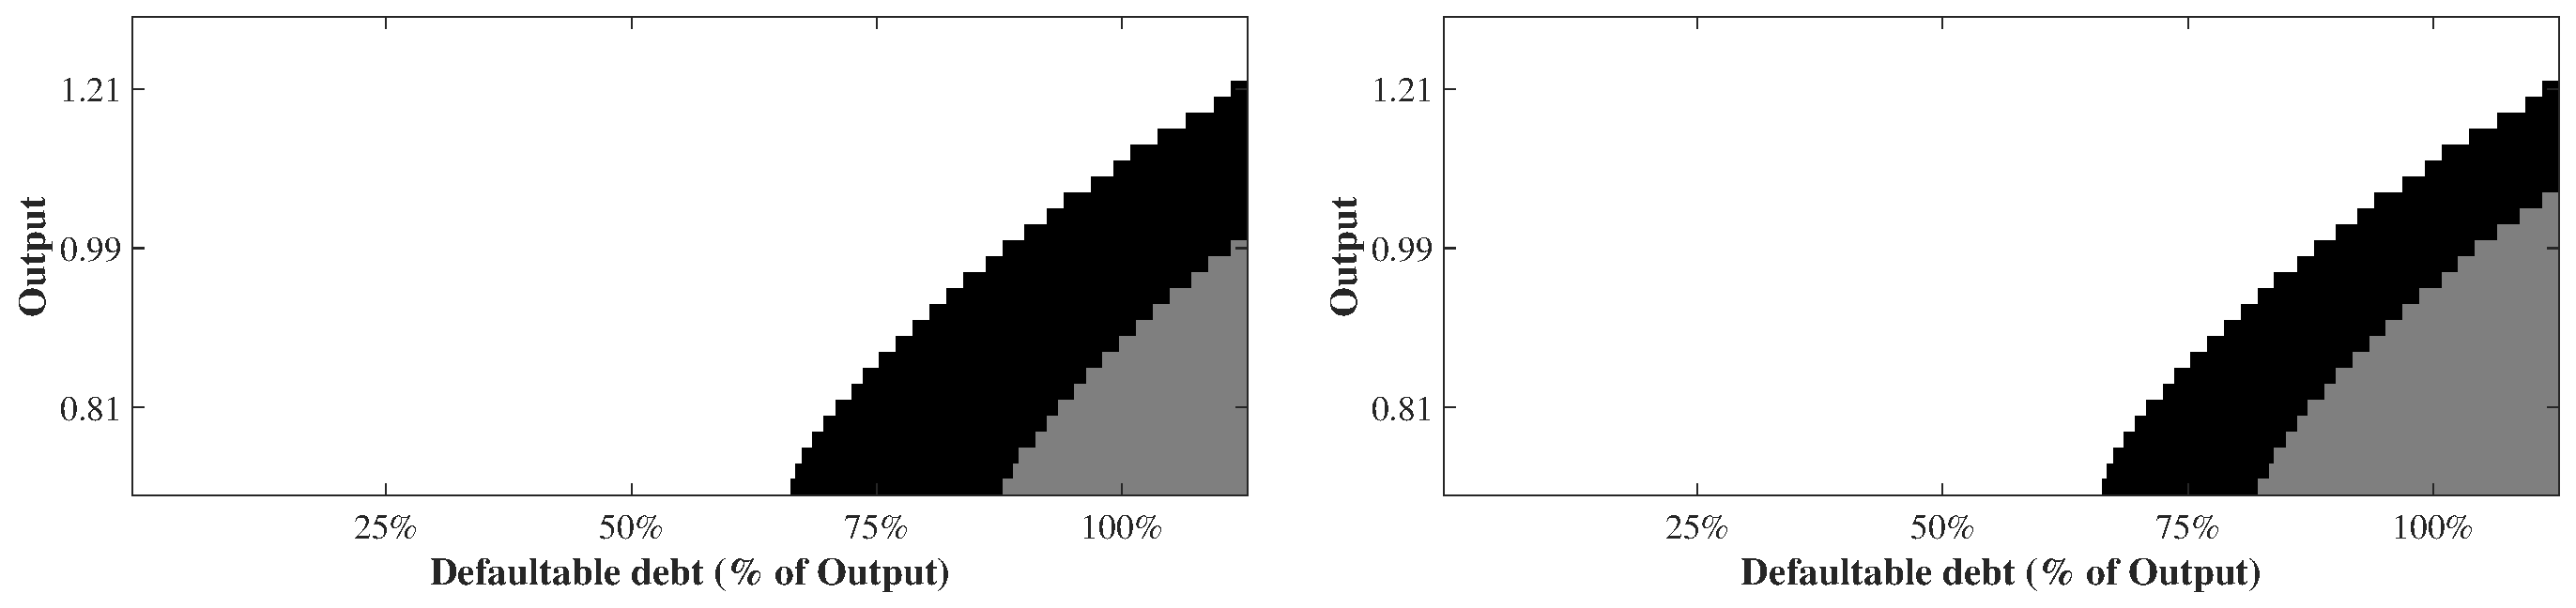
\includegraphics[scale=0.27]{default_decision_alpha55.eps}
    }
        \begin{tablenotes}
      \footnotesize
    Figure A.1 shows the default decision matrix for an economy without (black area) and an economy with Eurobonds (gray area). The left panel displays the decision where for both economies $e = 0$. The right panel shows the default decision where both economies are at their non-defaultable debt limit, $e = 0$ and $e = 0.4$ respectively.
    \end{tablenotes}
\end{figure}
\vspace{11mm} 
\begin{figure}[H]
\caption{\textbf{Default decision for $\bm{\alpha = 0.65}$}}
    \centering
    \vspace{1mm}
     \resizebox{\columnwidth}{4.6cm}{%
   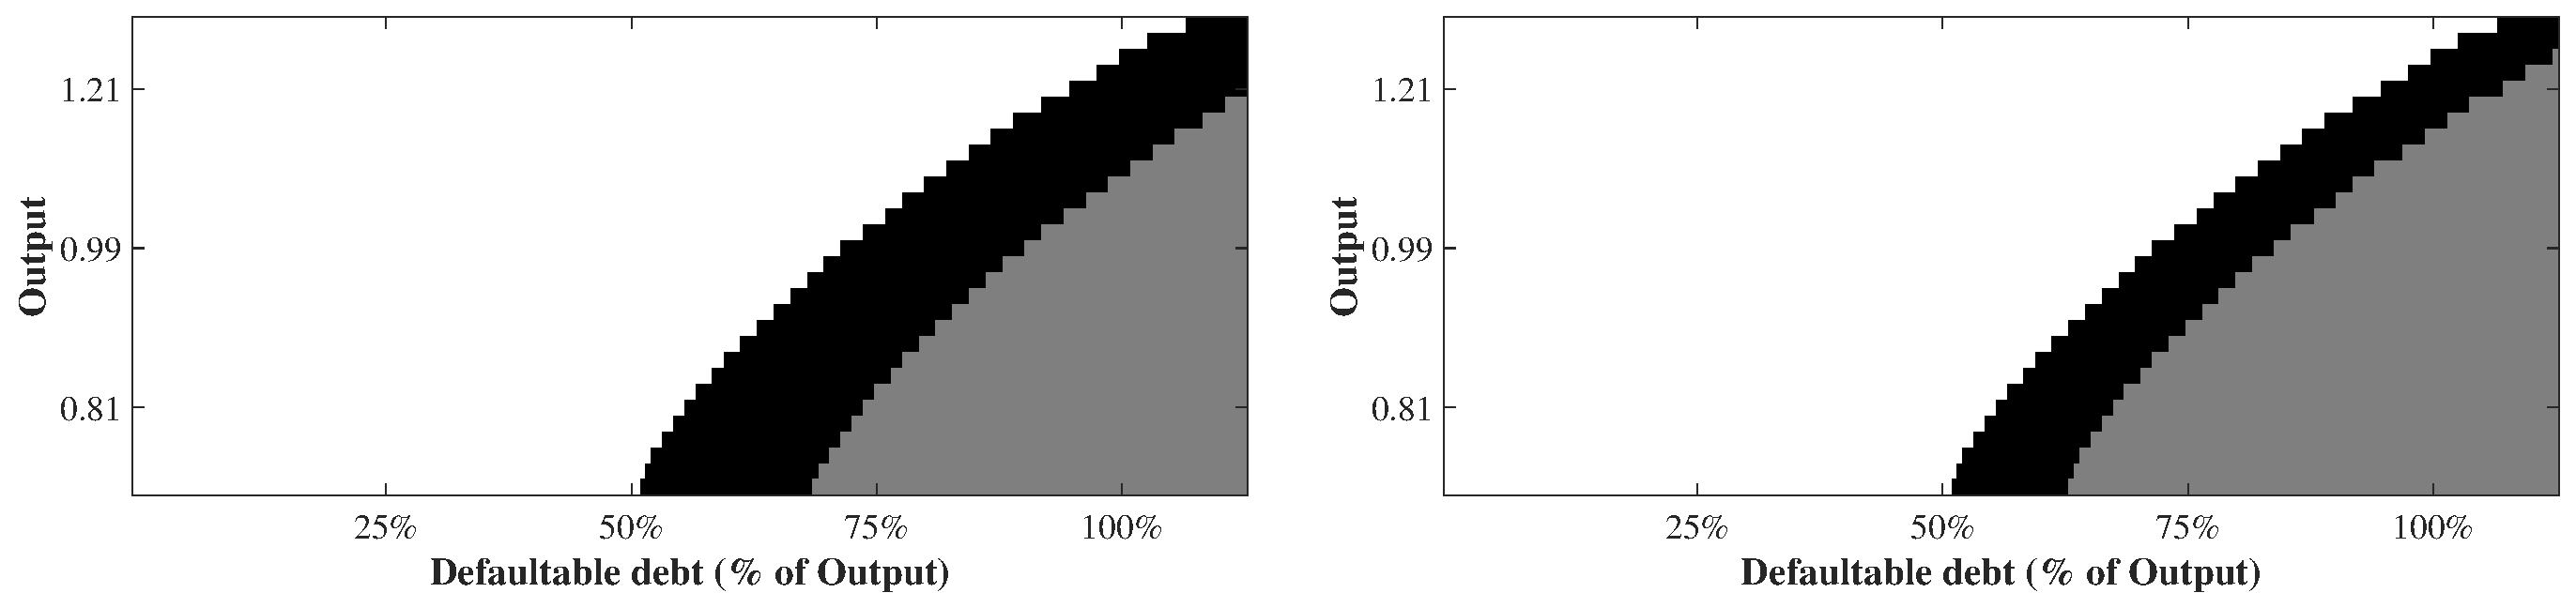
\includegraphics[scale=0.27]{default_decision_alpha65.eps}
    }
        \begin{tablenotes}
      \footnotesize
    Figure A.2 shows the default decision matrix for an economy without (black area) and an economy with Eurobonds (gray area). The left panel displays the decision where for both economies $e = 0$. The right panel shows the default decision where both economies are at their non-defaultable debt limit, $e = 0$ and $e = 0.4$ respectively.
    \end{tablenotes}
\end{figure}

\begin{figure}[H]
\caption{\textbf{Default decision for $\bm{\alpha = 0.75}$}}
    \centering
    \vspace{1mm}
     \resizebox{\columnwidth}{4.6cm}{%
   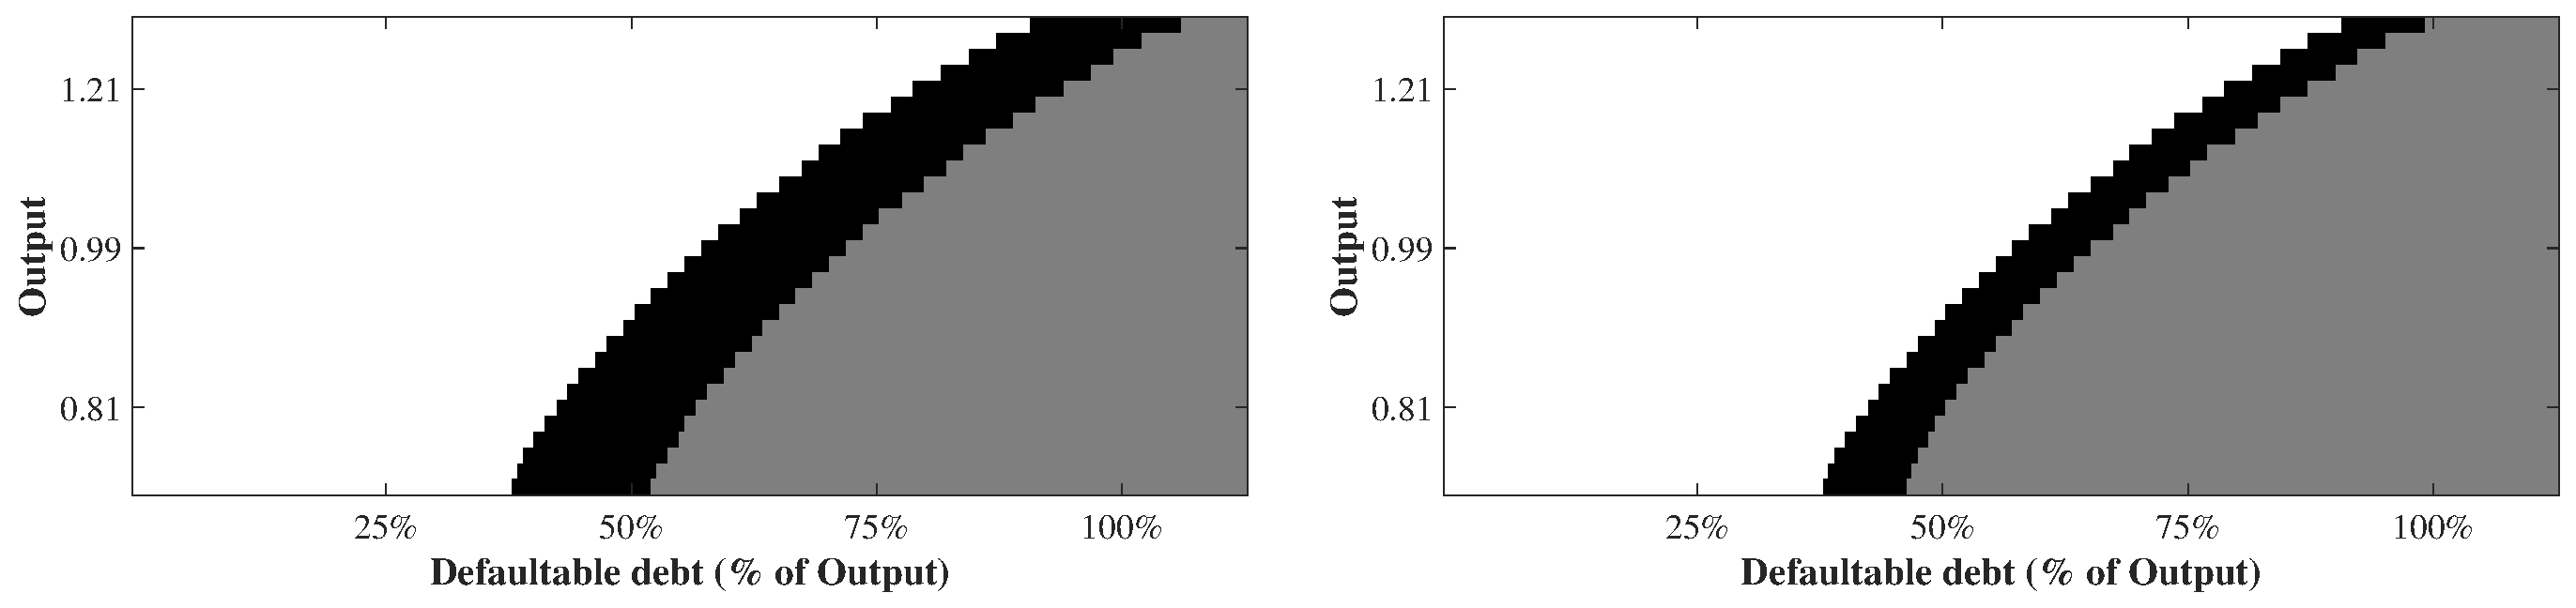
\includegraphics[scale=0.27]{default_decision_alpha75.eps}
    }
        \begin{tablenotes}
      \footnotesize
    Figure A.3 shows the default decision matrix for an economy without (black area) and an economy with Eurobonds (gray area). The left panel displays the decision where for both economies $e = 0$. The right panel shows the default decision where both economies are at their non-defaultable debt limit, $e = 0$ and $e = 0.4$ respectively.
    \end{tablenotes}
\end{figure}

\begin{figure}[H]
\caption{\textbf{Default decision for $\bm{\alpha = 1}$}}
    \centering
    \vspace{1mm}
     \resizebox{\columnwidth}{4.6cm}{%
   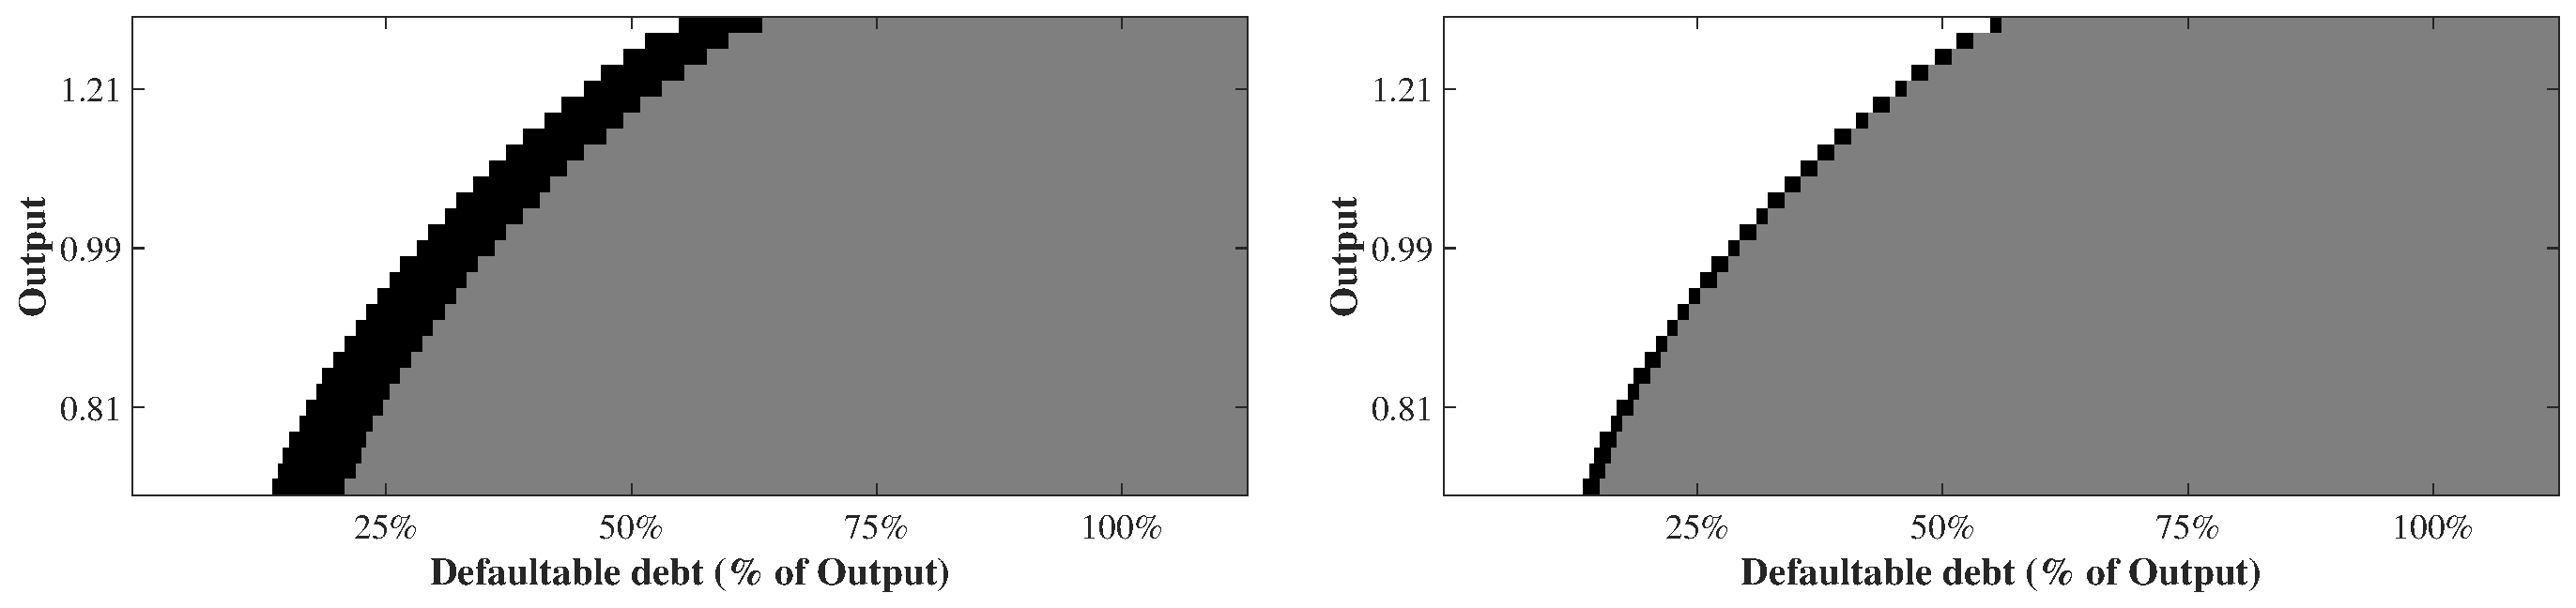
\includegraphics[scale=0.27]{default_decision_alpha1.eps}
    }
        \begin{tablenotes}
      \footnotesize
    Figure A.4 shows the default decision matrix for an economy without (black area) and an economy with Eurobonds (gray area). The left panel displays the decision where for both economies $e = 0$. The right panel shows the default decision where both economies are at their non-defaultable debt limit, $e = 0$ and $e = 0.4$ respectively.
    \end{tablenotes}
\end{figure}

\end{appendices}

\begin{appendices}
\chapter{Step-by-step guide to replicating the results}
This appendix goes over the step-by-step replication of the dissertation's results. All figures and tables are generated in \texttt{Matlab} and the \texttt{.m-files} to solve the model and run the simulations are based on Uribe \& Schmitt-Grohé's code which is available online\footnote{\url{http://www.columbia.edu/~mu2166/book/sovereign_debt/}}.\\

Before running the code, two comments should be taken into consideration. First of all, to improve \texttt{Matlab}'s efficiency in solving the model, defaultable debt and non-defaultable debt are treated jointly. This means that government debt is represented by a "bundle" of regular debt and Eurobonds. By doing so, we increase the computational efficiency in the maximization routines by treating the problem as a 2-dimensional instead of a 3-dimensional problem. A second remark to take into consideration is that solving for every calibration of the model can take up to 6 days or more, depending on your hardware specifications. The baseline model alone with Eurobonds can take 20 hours or more to solve. The smaller the grid size of the model, the lower the computation time and vice versa. All original \texttt{.mat-files} are available on request to immediately replicate the results from Step 3 (cf. infra).\\

To generate the results, the steps below need to be performed. It is imperative that between all \texttt{.m-files} the same names are used for the \texttt{.mat-files} in which the different solutions are stored. Certain \texttt{.m-files} require multiple inputs for which all names need to be adjusted accordingly. 
\begin{itemize}
    \item \textbf{Step 1:} Run \texttt{tpm.m} to generate the output grid and the transition matrix. The resulting \texttt{.mat-file} will be used as input for Step 2.
    \item \textbf{Step 2:} Run \texttt{egr\_nondef\_final.m} to solve the model through Value Function Iteration. This step needs to be repeated for every change made to the baseline calibration.
    \item \textbf{Step 3:} All tables and figures are generated by separate \texttt{.m-files}. Every first file in the following steps uses the generated \texttt{.mat-file} from Step 2.
    \begin{itemize}
        \item All tables are generated by running \texttt{simu\_regular.m} and \texttt{statistics.m} in this order. This step needs to be repeated for every different calibration.
        \item Figure \ref{fig:default decision} and Figures A.1-A.4 are generated by \texttt{Default\_decision.m} and uses 2 \texttt{.mat-files} as input: the first with Eurobonds and the second without Eurobonds.
        \item Figure \ref{fig:intro} is generated by running \texttt{simu\_intro.m} and \texttt{Introduction.m} in this order.
        \item Figure \ref{fig:default_episode} is generated by running \texttt{simur\_regular.m} and \texttt{default\_episode.m} in this order.
        \item Figure \ref{fig:intro_comp} is generated by running \texttt{simu\_intro.m} and \texttt{intro\_comp.m} in this order. The file \texttt{simu\_intro.m} needs to be run five times for each separate calibration.
        \item Figure \ref{fig:intro_debtrule} is generated by running \texttt{simu\_intro.m} and \texttt{intro\_comp\_debtrule.m} in this order. The file \texttt{simu\_intro.m} needs to be run four times for each separate calibration.
        \item Figure 3.6 and 3.7 are generated by running \texttt{multiplicity.m} which uses two \texttt{.mat-files} as input: the standard baseline model and the bad equilibrium model.
    \end{itemize}
\end{itemize}
\end{appendices}






%Eind
\newpage
\thispagestyle{empty}
\newgeometry{textwidth=540pt,textheight=780pt,top=20pt,left=20pt,right=20pt}
\begin{figure}[ht]
\begin{flushright}

\includegraphics[width=0.5\textwidth]{Picture3.png}	
\end{flushright}
\end{figure}
\vfill
\begin{picture}(550,40)
\put(0,0){\colorbox{kuleuven}{\makebox(520,52){}}}
\end{picture}
\end{document}